\documentclass[10pt, conference, compsocconf]{IEEEtran}
\ifCLASSINFOpdf
\else
\fi
\hyphenation{op-tical net-works semi-conduc-tor}
\usepackage[dvips]{graphicx}
\usepackage{xcolor}
\usepackage{cite}
\usepackage{array}
\usepackage{makecell}
\usepackage{subfig}
\usepackage{fancybox}
\usepackage{comment}
\usepackage[cmex10]{amsmath}
%\usepackage[tight,footnotesize]{subfigure}

\def\Correction{\color{blue}}
\newcommand{\Corr}[2]{\GF{#1} {\Correction #2}}

\begin{document}
%\title{Short paper:\\Body Biasing Injection: Best practices, attack and fault model}
\title{A better practice for Body Biasing Injection}
\author{\IEEEauthorblockN{G. Chancel, J.-M. Galliere, P. Maurine}
        \IEEEauthorblockA{University of Montpellier, LIRMM\\
                            Montpellier, France\\
                            Email: gchancel@lirmm.fr}}

% \author{\IEEEauthorblockN{XXXX.XXXX}
%        \IEEEauthorblockA{XXXX, XXXX\\
%                            XXXX, XXXX\\
%                            Email: XXXX@XXXX.XXXX}}
\maketitle

\begin{abstract}
Body Biasing Injection (BBI) is a fault injection method involving applying a voltage pulse onto the backside substrate of integrated circuits using a conductive needle.
Some studies have been focusing on the characterization of BBI effects, but no fault model explaining the origin of the induced faults has yet been established.
The repeatability of this method has been demonstrated, and electrical models have been proposed. However, up to the best of our knowledge, no successful differential fault attack using BBI and single bit fault model on hardware coprocessors has yet been reported in the literature.
Within this context, this work presents enhanced practices to perform BBI in an even more reproducible and reliable way compared to previous works.
It also brings insights on how and why faults occur under BBI and presents a fault attack performed on a hardware AES coprocessor embedded in a modern 32-bits microcontroller.

\end{abstract}

\begin{IEEEkeywords}
Body Biasing Injection; Fault Injection; Fault Attack; Fault model
\end{IEEEkeywords}
\IEEEpeerreviewmaketitle

%%%%% PARTIE 1 : INTRO %%%%%
\section{Introduction}
\label{section:intro}
There are several hardware-based fault injection techniques to perform attacks on integrated circuits (ICs), such as power glitch injection \cite{powerGlitch}, laser fault injection (LFI) \cite{optical, phototriple, lfitriplewell}, electromagnetic fault injection (EMFI) \cite{mathieuEMFI, techEM}, but also the one discussed in this work: Body Biasing Injection (BBI) \cite{pmaurine2012, japBBI, oflynn2020, nbb2016, ktobich2013}, not to mention all of them.

BBI involves applying a positive or negative voltage pulse onto the substrate of ICs with a conductive needle.
It works thanks to the IC conductive structure, which is roughly a stack composed of a block of P-doped silicon (the substrate), the logic gates, and a network of metals connecting and powering the logic gates.
The substrate being mostly a resistive environment, electrical charges can flow up or down through it, depending on the pulse polarity, to the logic gates and the power delivery network.

Unlike LFI or EMFI, there is little knowledge about BBI in the literature, and therefore, there are still many things to unveil.
For instance, currently, there are only a few insights on how faults occur in ICs subject to BBI but also on the characteristics of the induced disturbances.

This explains why in this work we intend to improve existing techniques for performing BBI using coarse platform models.
We then compare the models' simulation results to real measurements.
Next, we confront the obtained simulation results with real measurements.
% The simulation results obtained with these models are then compared to real measurements.
Afterward, fine-tuned complex IC models, similar to \cite{mybbi1} and \cite{mybbi2}, are introduced to identify a fault model.
Eventually, we demonstrate the proposed BBI platform enhancements efficiency by applying Giraud's differential fault attack, requiring single-bit faults to be successful, on a hardware AES coprocessor embedded in a modern 32-bits microcontroller.
% Eventually, the efficiency of the proposed BBI practice is demonstrated by applying Giraud's differential fault attack, which requires single-bit faults to be successful, on a hardware AES coprocessor embedded in a modern 32-bits microcontroller.
It is, up to the best of our knowledge, the first BBI based DFA on a hardware coprocessor reported in the literature.

%%%%% PARTIE 2 SOUS-PARTIE B : Real XP %%%%%
\label{subsection:simpleXP}
\begin{figure}
\centering
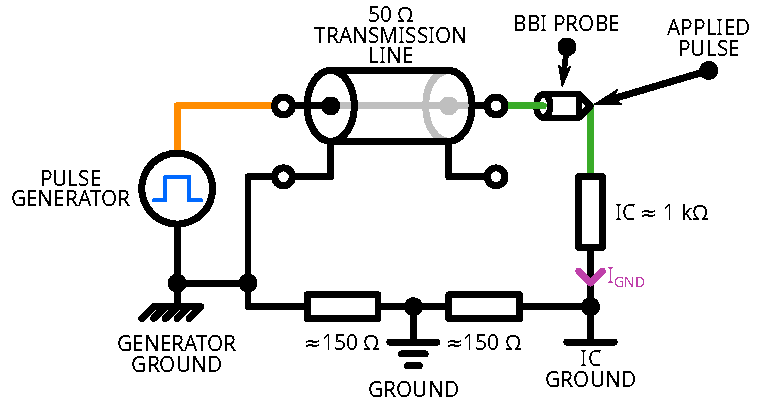
\includegraphics[width=3in]{model0Probe}
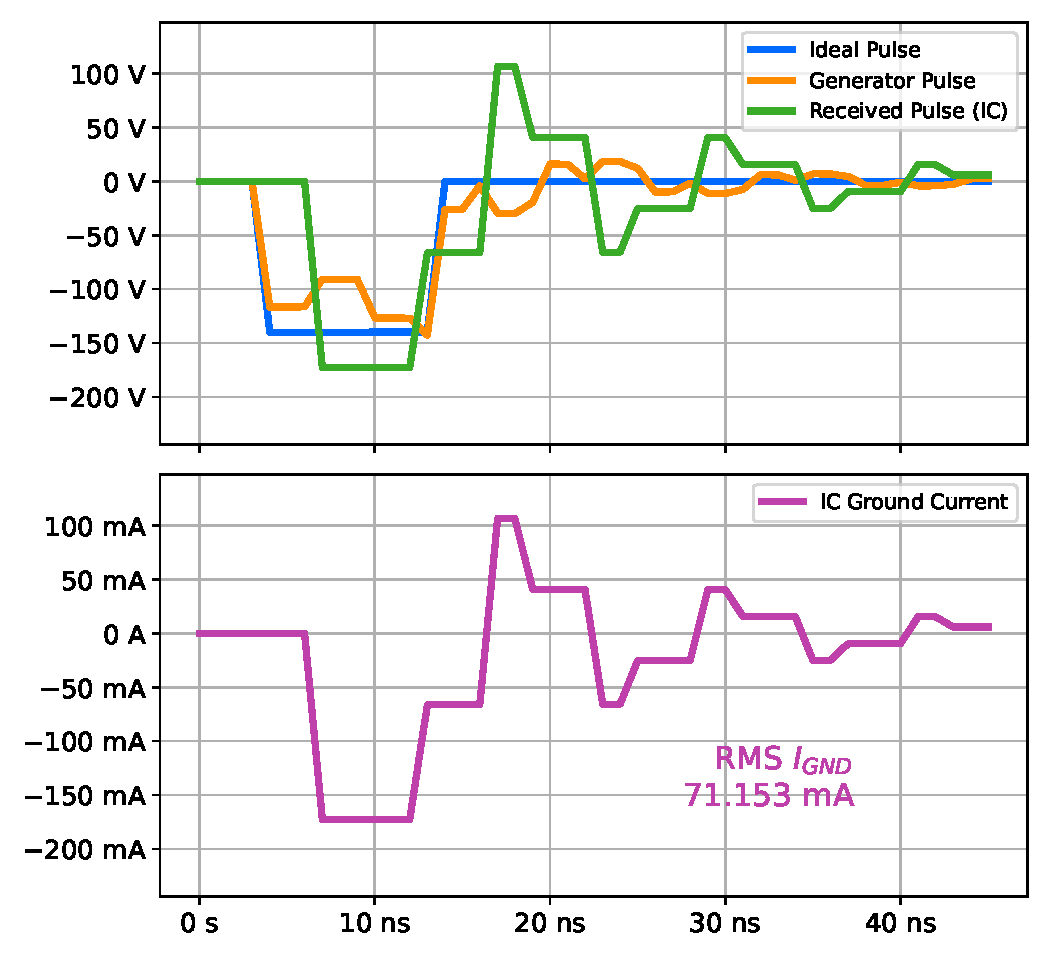
\includegraphics[width=3in]{SIMPLE_BBI_0.pdf}
\caption{Body Biasing Injection in the state of the art – Scenario 1}
\label{simpleModel0}
\end{figure}


\begin{figure}[hbtp]
\centering
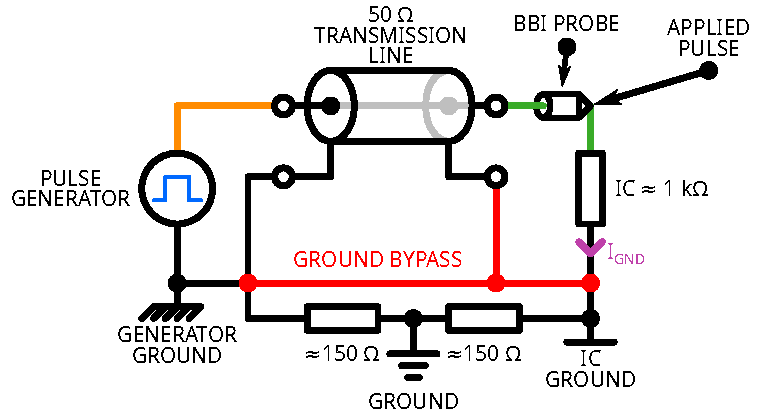
\includegraphics[width=3in]{model1Probe}
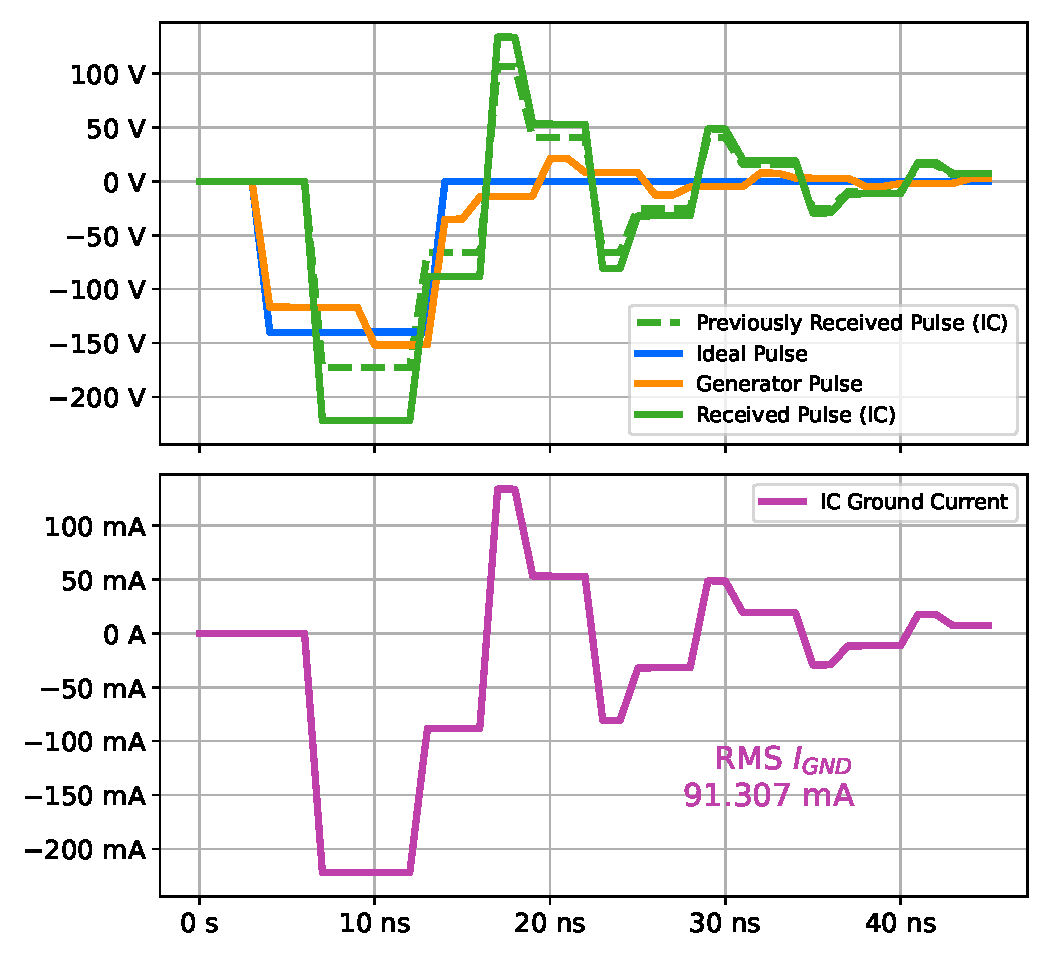
\includegraphics[width=3in]{SIMPLE_BBI_1.pdf}
\caption{Body Biasing Injection with proper equipment grounding – Scenario 2}
\label{simpleModel1}
\end{figure}

\begin{figure}[hbtp]
\centering
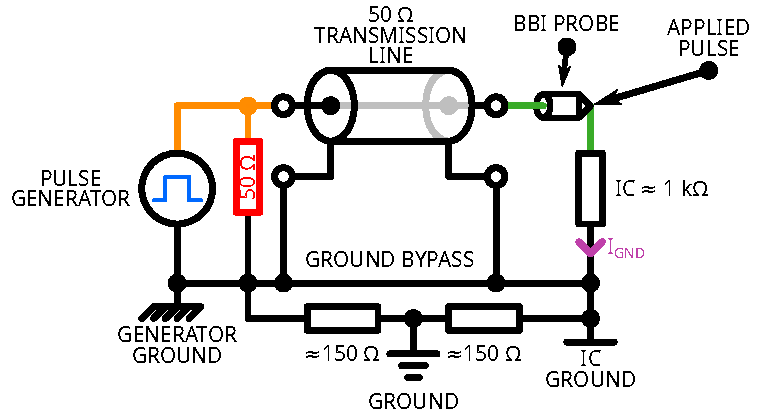
\includegraphics[width=3in]{model2Probe}
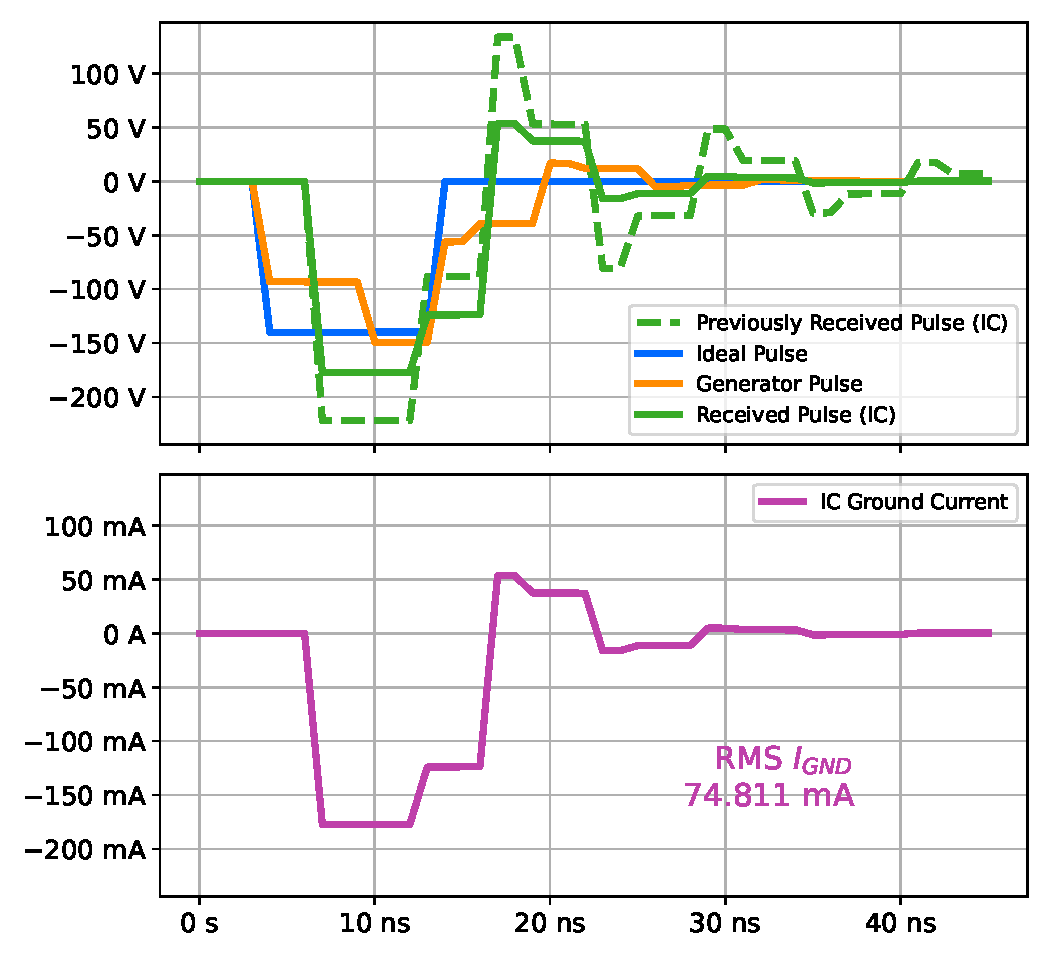
\includegraphics[width=3in]{SIMPLE_BBI_2.pdf}
\caption{Body Biasing Injection with proper equipment grounding and impedance matching – Scenario 3}
\label{simpleModel2}
\end{figure}

%%%%% PARTIE 2 : Explications des bonnes pratiques %%%%%
\section{BBI: Better practice explained with coarse electrical models}
\label{section:simpleModel}
Simulating ICs electrical behavior under BBI has been first proposed in \cite{mybbi1} and was further studied in \cite{mybbi2}.
In both of these works, elaborated electrical models were proposed to evaluate the effects of thinning the substrate, and then to characterize the electrical disturbances appearing inside ICs under BBI for both dual-well and triple-well substrate type.
It was demonstrated that thinning the substrate allows reducing the minimal voltage pulse amplitude required to induce faults, while also reducing the IC response times to those pulses.
Therefore, thinning the substrate improves the time control an attacker has over ICs under BBI.
In addition to this, depending on the substrate type and the voltage pulse polarity, it has been shown that the coupling between the injection probe and the logic gates differs, which then changes how ICs behave when subject to BBI.

Within this context, this section aims at introducing enhanced BBI platforms to achieve more accurate (both in time and space) and more reproducible fault attacks using BBI.
In the first place, we analyze the proposed platforms using electrical simulations.
% The analysis of the proposed platforms is first achieved using electrical simulations.
For simplicity, coarse models of BBI platforms and triple-well ICs (present in ICs designed with modern technologies) were used during these simulations.
To demonstrate the soundness of the examined BBI practices, we compare the obtained simulation results to equivalent experimental ones.
Eventually, because the fundamental objective is to achieve exploitable fault injection, we perform and analyze the results of an actual Giraud's DFA on a modern microcontroller for each platform.
% Eventually, because the fundamental objective is exploitable fault injection, the results of a real Giraud's DFA obtained on a modern microcontroller with each practice were compared.

%%%%% PARTIE 2 SOUS-PARTIE A : Overview %%%%%
\subsection{Different practices of BBI}
\label{subsection:simpleModels}
For improving the understanding of BBI in addition to presenting the enhanced BBI platforms we propose, let us examine three coarse BBI platforms electrical models, solely considering their most significant macro parameters.
% For the purpose of improving the understanding of the BBI but also to present the enhanced practices of BBI the paper proposes, let us examine three coarse models of three slightly different BBI platforms which only consider their most significant macro parameters.
These three models, denoted straightforwardly scenarios 1, 2 and 3 in the rest of the paper, are shown respectively in Fig. \ref{simpleModel0}, \ref{simpleModel1} and \ref{simpleModel2}.
As illustrated, in every case, a BBI platform model features:
\begin{itemize}
\item A high voltage pulse generator
\item A $50 \; \Omega$ transmission line (SMA cable) 
\item A BBI probe
\item An IC modeled by a $1\:k\Omega$ resistor
\item The platform ground modeled by two $150\:\Omega$ resistors (measured in our test setup)
\end{itemize}
In Fig. \ref{simpleModel0}, \ref{simpleModel1} and \ref{simpleModel2} are also depicted the waveforms of important signals obtained by simulation to analyze the efficiency of the proposed BBI platforms enhancement.
These signals are, in order of occurrence:
\begin{itemize}
\item The waveform of the ideal voltage pulse applied to the substrate
\item The waveform of the voltage pulse generator output
\item The waveform of the voltage applied to the IC backside
\item The waveform of the IC ground current
\end{itemize}
The first scenario shown in Fig. \ref{simpleModel0} depicts the way BBI has been performed since its first documented use in \cite{pmaurine2012}.
This setup has two main flaws, which are presented in the next paragraphs.

\subsection{Improper grounding}
First, due to the inherent nature of a BBI platform equipment, which can greatly vary from one platform to another, as described in Fig. \ref{simpleModel0}, it is difficult to choose a correct and stable voltage reference, in other words a ground, for measurements and settings.
For instance, the current flowing from the pulse generator to the global ground through the $150 \; \Omega$ resistors during an injection, shifts (reduces or increases) the amplitude of the voltage applied to the BBI probe according to the pulse polarity.
This effect limits the repeatability of results from one BBI platform to another, and even from a board embedding the same IC target compared to another board.

Instead, as it has been proposed in \cite{mybbi2}, it is preferable to choose the ground of a piece of equipment as a common voltage reference to all devices and thus shunting the original platform ground using low-resistance interconnections, such as short and thick copper wires, as illustrated in Fig. \ref{simpleModel1}.

By doing so, the global ground impedance is widely reduced in most cases, thus allowing for more electrical charges to go through and potentially interact with the IC logic gates.
The RMS current going out of the IC ground sees a $28 \: \%$ increase in that case, as shown in Fig. \ref{simpleModel0} and \ref{simpleModel1}).
% Later in this work, we demonstrate that in can ease and sometimes enables fault creation for a same set of input parameters.

\subsection{Impedance mismatch}
Despite this first enhancement, a significant problem remains with both of these setups.
Indeed, when observing the signals in Fig. \ref{simpleModel0} and \ref{simpleModel1}, it is easy to notice significant ringing on both the voltage pulse applied to the substrate and the current going out of the IC ground.

The ringing on the transmission line (in that case a $30 \; cm$ long SMA cable) is due to the impedance mismatch between the IC and the voltage pulse generator (usually designed to control a precise electrical charge, typically $50 \; \Omega$).
It acts by limiting the power transfer from the generator to the IC target and by reducing the BBI time resolution.
Indeed, the induced disturbances are much longer (more than three times in the simulation) than that of the pulse an adversary might want to apply.

In numerous instances, IC substrates do not have the exact required impedance for generators nor a constant impedance over their entire backside surface.
Indeed, we experimentally observed that the latter varies from a BBI probe position to another, as we describe in the next paragraph.
% Indeed, it has been experimentally observed that the latter varies from a BBI probe position to another, as described in the next paragraph.
As a result, the voltage pulse generator input settings (voltage amplitude and pulse width) cannot be met without further modification of the platform.
This is problematic when comparing results obtained on different platforms, or even on a unique platform.
For instance, just changing the length of the transmission line (SMA cable) can drastically change the required settings to induce a fault or to reproduce an experiment.

To overcome this issue, we suggest connecting a resistive compensation load (in that specific case, a $50 \; \Omega$ load) at the output of the voltage pulse generator in parallel to the targeted IC to place the aforementioned generator closer to its specified operating conditions.
By doing so, one can remark in Fig. \ref{simpleModel2} a significant ringing amplitude and number reduction in both the applied pulse and the IC ground current.
As a result, the pulse applied to the IC is closer to the requested pulse.
Thus, this enhancement provides enhanced control and repeatability of BBI, and above all, increases the time resolution of BBI which can be of great help to perform successful DFA.

It is worth noting that connecting the compensation load before the transmission line as we suggest and show in Fig. \ref{simpleModel2} is far from ideal.
It would be better to connect it at the output of the transmission line, closer to the target IC.
However, we prefer to suggest the first solution because it is technically easier as it requires almost no modification to an existing setup and provides a low-cost and sufficient approximate impedance matching for the practice of BBI.
Thus, we will evaluate this solution for the rest of the work.

\begin{figure}[!h]
\centering
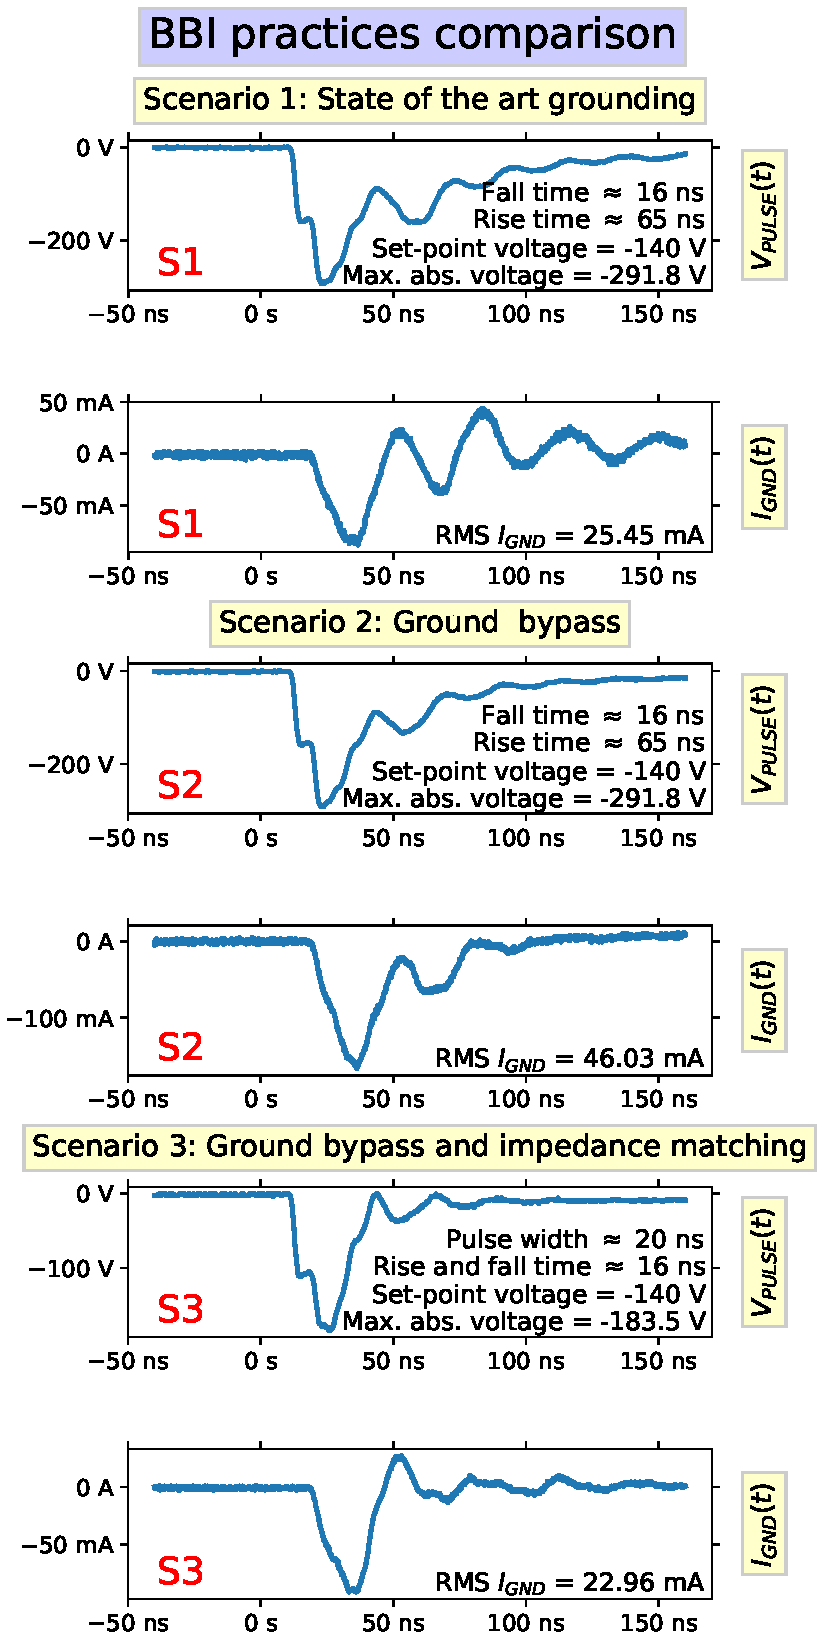
\includegraphics[width=3in]{realPulsesComparisons.pdf}
\caption{Waveforms of the voltage pulse and the IC ground current respectively, measured at the output of the generator and at the ground pad of the IC respectively}
\label{pulseIgndAll}
\end{figure}

\section{Good practice of BBI:  preliminary experimental results}
To compare experimentally the different scenarios, we carried out experiments aiming at reproducing the previous simulations with actual equipment.
Afterward, we will introduce the test bench used for all experiments.
% To experimentally compare the different scenarios, we carried out, in the first place, experiments consisting in reproducing with actual equipment the previously described simulation results.
% Then, we will introduce the test bench used for all experiments.

% To experimentally compare the different scenarios, the first carried out experiments consisted in reproducing the simulation results described in the previous section with real equipment. The next paragraphs introduce the test bench used for all experiments.

%%%%% PARTIE 2 SOUS-PARTIE B SOUS-SOUS-PARTIE 1 : XP SETUP %%%%%
\subsection{Experimental setup}
\label{subsubsection:labSetup}

The platform is composed of a microcontroller manufactured with a $90 \; nm$ technology node using an ARM Cortex M4 CPU core.
It contains $256 \; kBytes$ of RAM, $2 \; MBytes$ of FLASH memory organized in two independent banks, and an embedded security coprocessor.
The microcontroller has been clocked at $40 \; MHz$ in all experiments, and its substrate thickness measures about $750 \; \mu m$.
The voltage pulse generator is an AVRK-4B-PN manufactured by Avtech Electrosystems Ltd.
It can generate various voltage pulses ranging from $50 \; V$ to $780 \; V$ with both negative and positive polarities.
Its pulse width ranges from $4.5 \; ns$ to $22 \; ns$, with fixed rise and fall times of $4 \; ns$ when optimally loaded with $50 \; \Omega$.

%%%%% PARTIE 2 SOUS-PARTIE B SOUS-SOUS-PARTIE 1 : XPs %%%%%
\subsection{Experiments}
\label{subsubsection:expSimple}

As it has been mentioned in \cite{mybbi1} and \cite{mybbi2}, BBI pulses with positive polarity tend to destroy in a few hours ICs under test.
Therefore, we only considered negative pulses in the rest of the paper.

For each real scenario, the requested pulse characteristics are the following:
\begin{itemize}
\item An amplitude of $- \; 140 \; V$
\item A pulse width of $20 \; ns$
\item Fixed rise and fall times of $4 \; ns$
\end{itemize}
Fig. \ref{pulseIgndAll} depicts the experimental results.
For each scenario, two signals are displayed: the voltage pulse effectively generated at the input of the transmission line and the current flowing out of the IC ground pin.
Each signal is labeled S1, S2, or S3 for better readability according to which scenario it is extracted from.
Moreover, the main characteristics of the applied pulses are annotated under the waveforms.

In the first scenario, we can observe that the effective pulse amplitude is more than twice the requested amplitude.
It can be explained because ringing is appearing on the signals due to an impedance mismatch between the generator and the microcontroller.
Ringing is specifically visible on the current waveform.
Eventually, the disturbance pulse width measures more than $125 \; ns$, which is more than six times the requested value of $20 \; ns$.
The discrepancies between the pulse generator settings and the effectively applied pulse to the IC can be worse or better depending on the impedance of the device under test.
However, the latter has no chance to be equal to $50 \; \Omega$ in practice.

Similar to what has been observed in the previous simulations, the results related to the second scenario show that a proper grounding of the platform almost doubles the current flowing out of the microcontroller ground.
In practice, the grounding we propose is first achieved by choosing an arbitrary piece of equipment ground as a voltage reference.
Then, from this ground to every other piece of equipment ground, short and low-resistance wires are connected.
However, if ringing is reduced concerning the ground waveform, this improvement does not significantly alter the pulse shape.
The disturbance still lasts, as expected from previous simulation results, for more than $125 \; ns$ due to the uncorrected impedance mismatch.

Eventually, results from the third scenario demonstrate that the impedance matching provides a drastic ringing reduction while allowing the pulse width and the pulse amplitude to be much closer to their respective requested values.

As a result, the current waveform almost follows the voltage pulse waveform with a slight delay (as shown in Fig. \ref{pulseIgndAll}) caused by the transmission line (the SMA cable and the microcontroller itself).
Additionally, we observe that the generator used is specified to deliver $4 \: ns$ rise and fall times, but even in the best case (the third scenario), the measured rise and fall times are four times higher than the specifications.
It can be explained because the ICs and transmission lines represent a complex impedance (RC load), which cannot be equated to a simple electrical resistance.
The generated pulses are thus shaped like an RC impulse response, and the pulse duration is roughly equal to $5\cdot RC$.

%%%%% PARTIE 3 : Expérimentations plus poussées et attaque %%%%%
\section{Further experiments and demonstrations}
\label{section:moreXP}

The previously described results being in line with the simulation results, we performed additional experiments to get insights on the impact of these enhancements on BBI platforms efficiency.
We conducted three kinds of experiments, consisting in plotting IC current injection maps and fault susceptibility maps, and most of all in performing a Giraud's differential fault attack.

%%%%% PARTIE 3 SOUS-PARTIE A: IMPEDANCE MAP %%%%%
\begin{figure}[!hbtp]
\centering
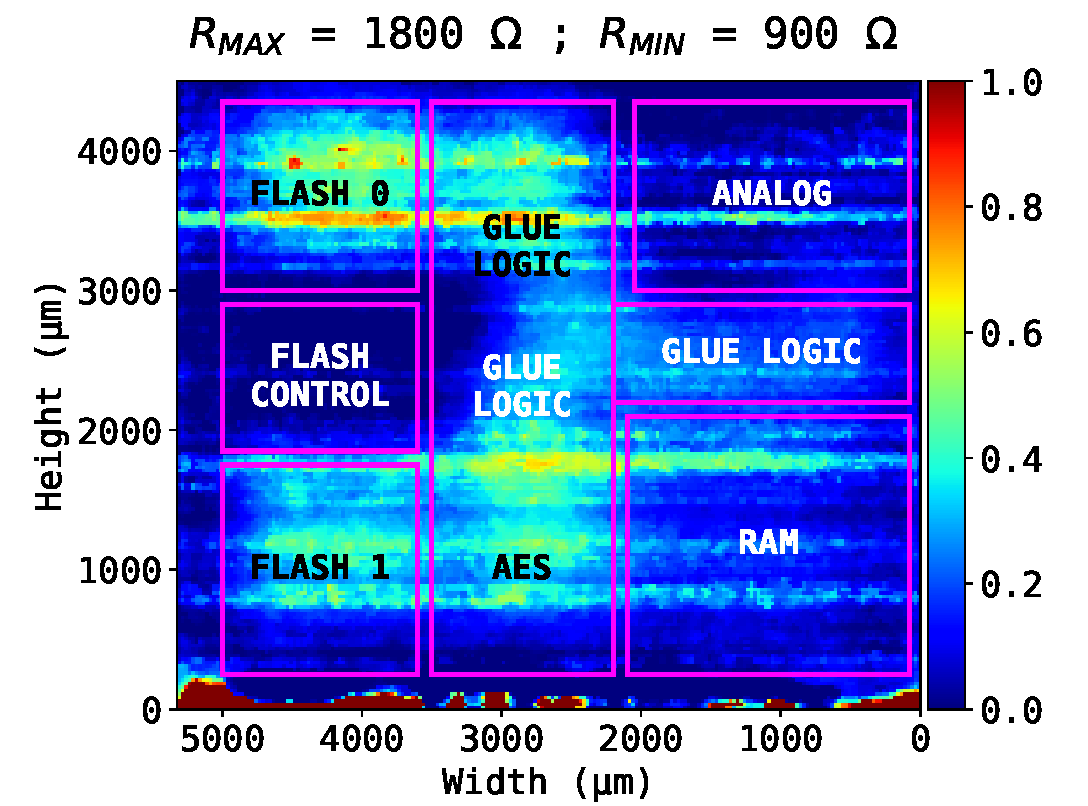
\includegraphics[width=3.35in]{resMap_M0}
\caption{Average normalized IC impedance mapping – Scenario 1}
\label{rCartos_M0_ignd}
\end{figure}

\begin{figure}[!hbtp]
\centering
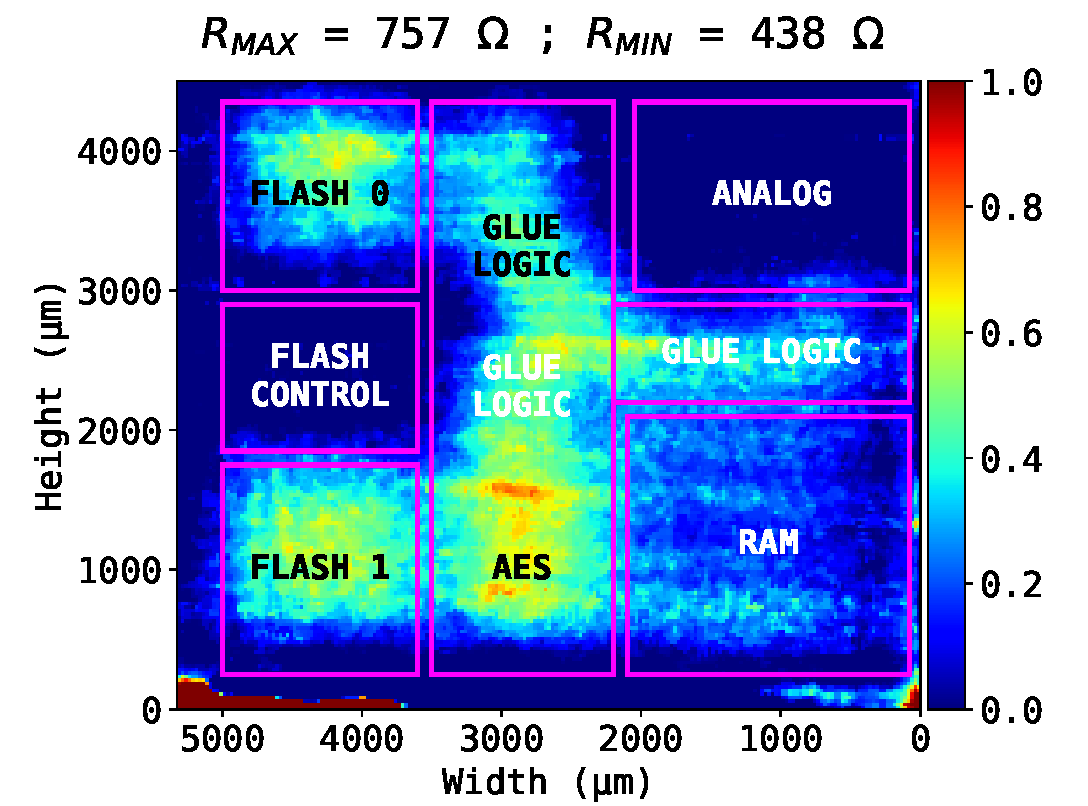
\includegraphics[width=3.35in]{resMap_M1}
\caption{Average normalized IC impedance mapping – Scenario 2}
\label{rCartos_M1_ignd}
\end{figure}

\begin{figure}[!hbtp]
\centering
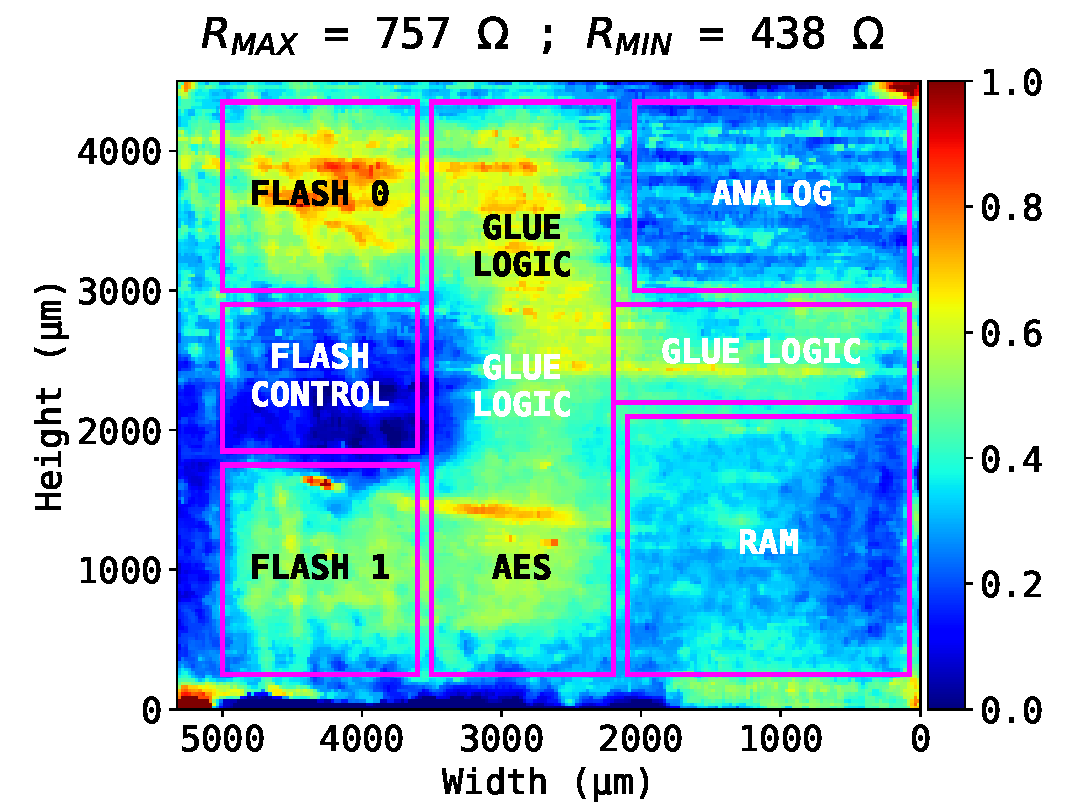
\includegraphics[width=3.35in]{resMap_M2}
\caption{Average normalized IC impedance mapping – Scenario 3}
\label{rCartos_M2_ignd}
\end{figure}

\subsection{IC impedance mapping}
\label{subsection:moreXPGLobalResMap}

In \cite{mybbi2}, it has been demonstrated that BBI can be used to get insights of the targeted IC floor plan by drawing a map of the current flowing out of the IC ground or power supply pin, according to the probe position.
Such maps were drawn with and without the two proposed enhancements.
The displacement step of the probe over the backside surface was set to $25 \; \mu m$ for each scan.
The pulse generator was set to generate a pulse of amplitude $- \;300 \; V$.
However, to be able to directly compare the different maps and because both applied voltage and ground current were measured, IC impedance maps ($Z \; = \; V \; \div \; I$) were drawn rather than IC current or voltage maps.

Fig. \ref{rCartos_M0_ignd}, \ref{rCartos_M1_ignd} and \ref{rCartos_M2_ignd} present the three maps after impedance normalization between their respective $R_{MIN}$ and $R_{MAX}$ to avoid any bias in the comparison due to the choice of the color scale. The comparison shows that:
\begin{itemize}
    \item The maps are quite similar and respectively highlight roughly the same low and high impedance areas, corresponding to areas where the substrate is respectively of dual-well type and triple-well type, the latter being where CMOS gates are usually lithographed.
    \item Bypassing the platform ground increases the injected current (scenario 2), and thus reduces the measured impedance compared to the first scenario.
    More precisely, it approximately halves the average measured IC impedance from about $1000 \; \Omega$ to $500 \; \Omega$.
    \item Matching the output impedance of the generator does not significantly alter the measured impedance (and thus the injected current), demonstrating that the injection strength main limiting factor is the BBI platform ground impedance (the two $150 \Omega$ resistors in Fig. \ref{simpleModel0}, \ref{simpleModel1} and \ref{simpleModel2}).
\end{itemize}
As we said before, it can be explained because ICs under BBI mainly behave as first order $RC$ low-pass filters.
The resistive component being roughly the sum of the substrate electrical resistance and the ground return path resistance.
The capacitive one being to the logic gates and the internal power supply network, both being mostly capacitive.
Thus, bypassing the ground return paths reduces the RC filter time constant and enables sharper and faster rise and fall times on both injected voltage and induced current waveforms on ICs under BBI.
This results in a significant improvement of the BBI time resolution.
%%%%% PARTIE 3 SOUS-PARTIE B: FSM %%%%%
\subsection{IC fault susceptibility mapping}
\label{subsection:moreXPGLobalFaultMap}

\begin{figure}[!hbtp]
\centering
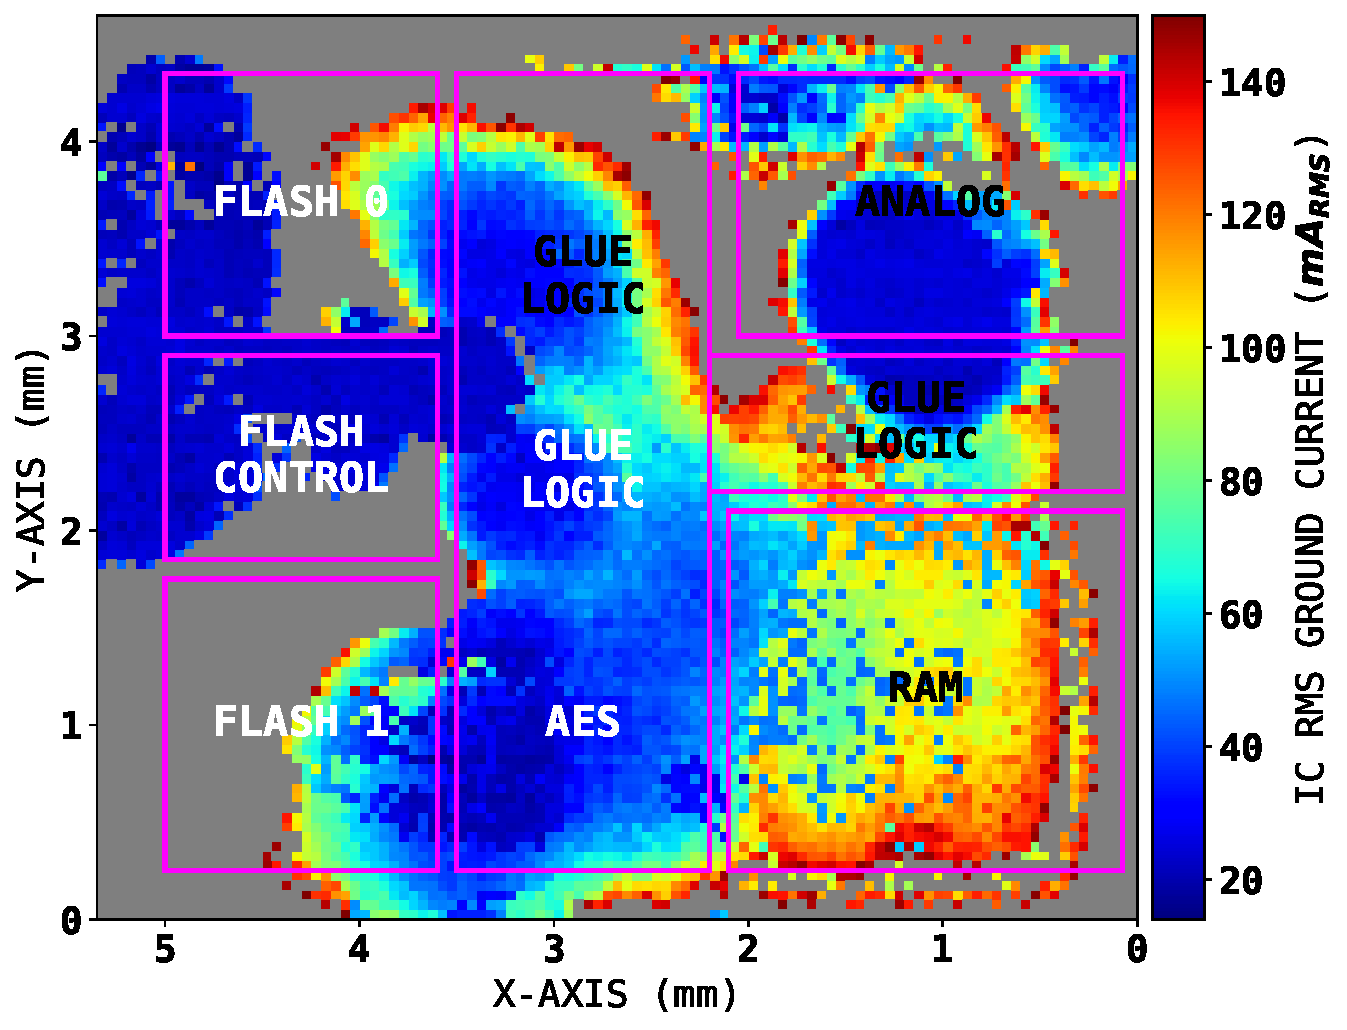
\includegraphics[width=3.35in]{aesBadGnd_C}
\caption{IC fault susceptibility mapping – Scenario 1}
\label{rCartos_M0_fault}
\end{figure}

\begin{figure}[!hbtp]
\centering
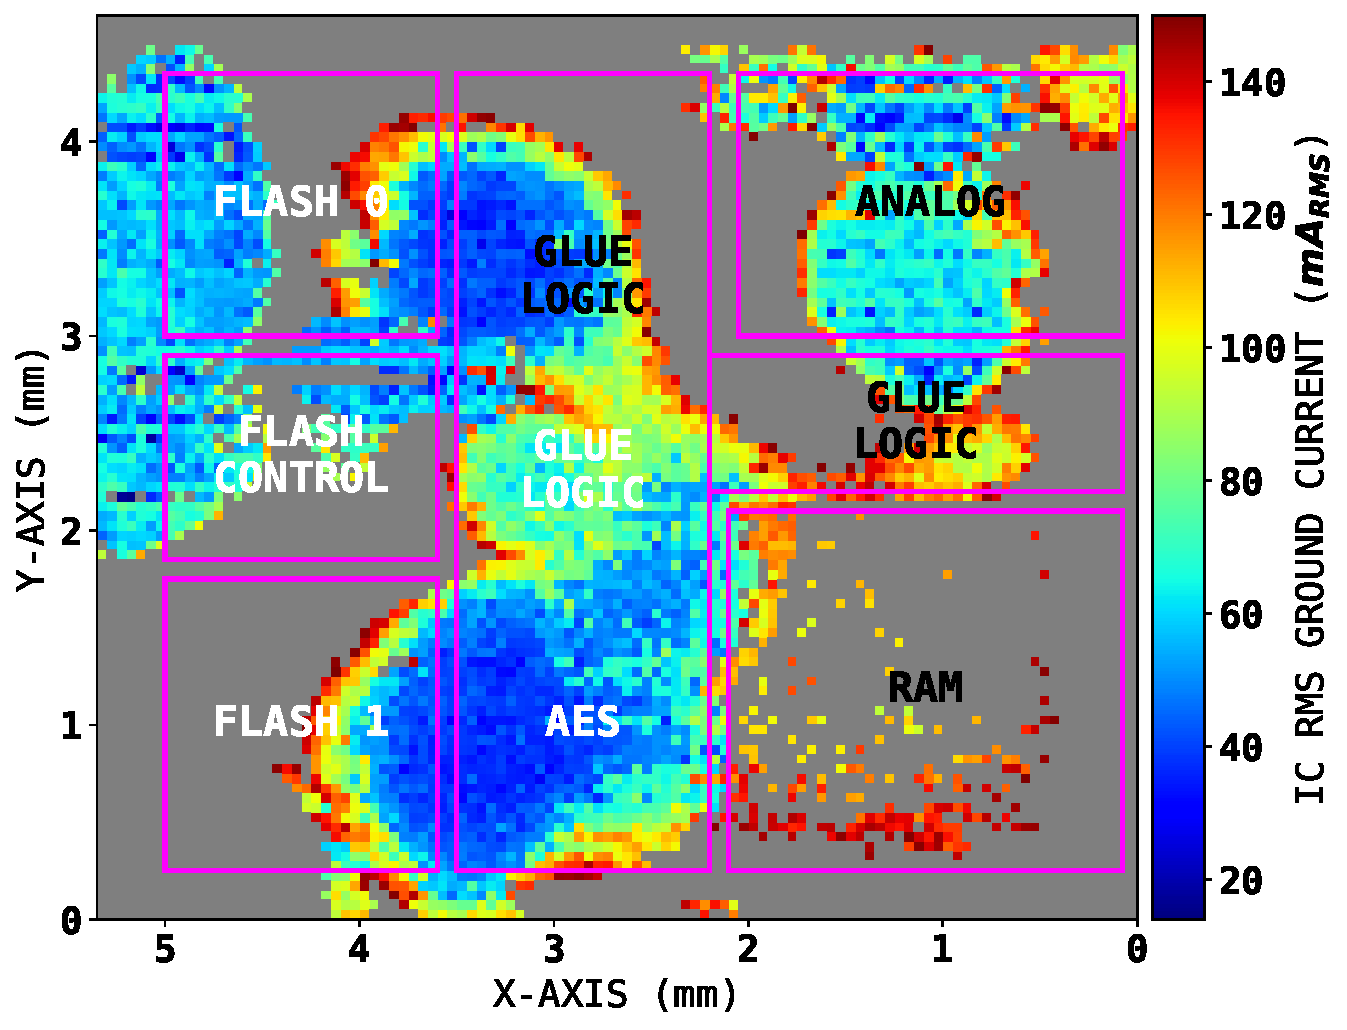
\includegraphics[width=3.35in]{aesGoodGndOnly_C}
\caption{IC fault susceptibility mapping – Scenario 2}
\label{rCartos_M1_fault}
\end{figure}

\begin{figure}[!hbtp]
\centering
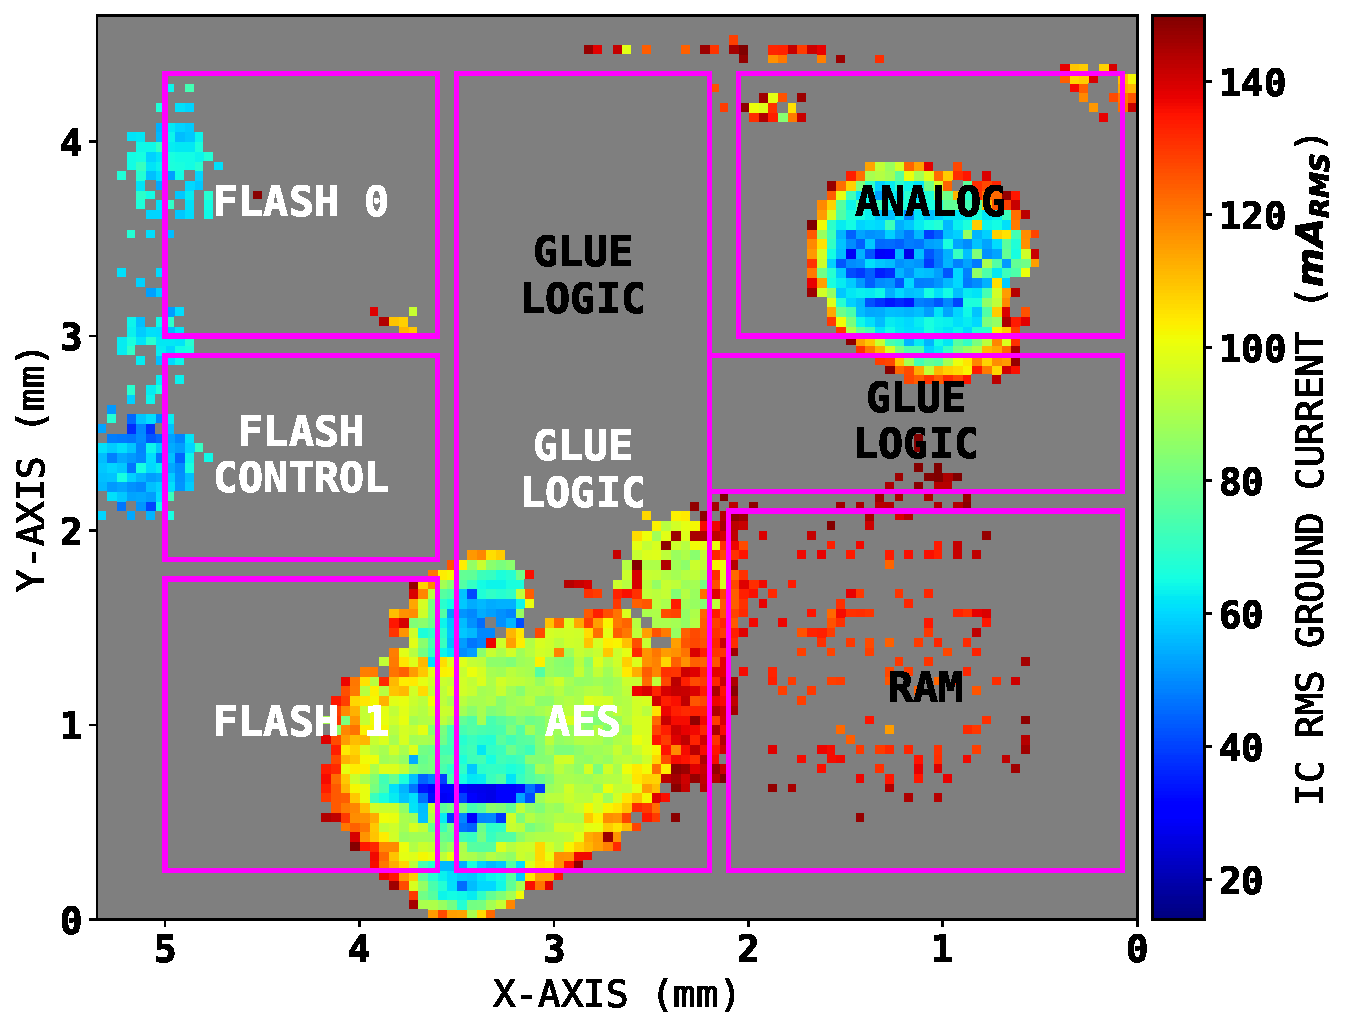
\includegraphics[width=3.35in]{aesBouchonGgnd_C}
\caption{IC fault susceptibility mapping – Scenario 3}
\label{rCartos_M2_fault}
\end{figure}

Similar to \cite{mybbi1}, IC faults susceptibility maps (FSM) were drawn and analyzed, as it is a valuable indicator of the efficiency of a fault injection method.
In \cite{mybbi1}, the BBI susceptibility was measured using the minimal voltage set-point of the generator, $V_{P}^{min}$, required to induce a fault at a given position of the probe on the backside of the IC.
Then, a map bringing together every measurement was drawn.
However, in this work, we decided to look at the minimal injected required current to induce a fault instead of the minimal set-point voltage.
Indeed, this allows to fairly compare the efficiency of the three different configurations of the BBI platform while it is more difficult when considering the $V_{P}^{min}$, mainly because the impedance seen by the generator changes at every position: on average $\approx 1.5 \; k\Omega $ in the first and historical configuration and $\approx 0.5 \; k\Omega $ in the second and third configurations.
Another reason explaining this choice comes from simulation results we describe in section \ref{section:attacks}, showing that the injected parasitic current is at the origin of the observed faults.

To that aim, a spatial scan of the entire IC was done with a probe travel step of $50 \; \mu m$.
The voltage range of the generator is different for each FSM, as it was adapted to never go above certain measured voltage and current to protect the IC.
The pulse width has been set to the maximum generator value of $22 \; ns$, and the penultimate AES round was the BBI time target to prepare the future DFA.
At each position, the IC behavior was analyzed and classified as:
\begin{itemize}
    \item Correct output: the IC provides a correct output.
    \item Type 1 faulty behavior: the IC provides a faulty output.
    \item Type 2 faulty behavior: the IC does not respond and crashes.
\end{itemize}
It is important to note that each time a faulty behavior of any kind was observed, the microcontroller was reset to eliminate any potential semi-permanent faulty behavior.
Additionally, it is important to remark that a type 1 faulty behavior does not necessarily mean that its result is exploitable when performing a fault attack.
Fig. \ref{rCartos_M0_fault}, \ref{rCartos_M1_fault} and \ref{rCartos_M2_fault} show the experimental FSMs.
The AES core is approximately located in the middle bottom half, as annotated in the Figures.

Concerning the first and second scenarios, we notice that faults are created when the probe is located above many functional areas: the AES, the analog blocks (PLLs and the voltage regulator…), the RAM, the FLASH, and the glue logic (CPU, UART…).
The induced disturbance, lasting more than $100 \; ns$ in both scenarios, seems to generate faults in different functional blocks operating at different times (clock cycles of $25 \; ns$ duration) after the computation targeted by the injection.
Thus, the poor time resolution of the BBI performed according to scenarios 1 and 2 results in a poor spatial resolution, as further blocks of the IC from the probe are disturbed.

That is not the case in the third scenario.
Indeed, faults are now mainly induced when the probe is above the AES and the analog blocks.
We think that the increase in observed spatial resolution is mainly due to the injection time resolution increase (reduction of the disturbance duration).
Indeed, as shown in Fig. \ref{pulseIgndAll}, the waveform of the injected current is sharper and lasts less than in scenarios 1 and 2, thus minimizing the risks of disrupting several clock cycles (lasting $25 \; ns$ each) and thus functional blocks involved throughout the algorithm.

It should also be noted that, in our case, properly grounding the platform (scenario 2) slightly increases the time and spatial resolutions of BBI (reducing the number of positions where faults are observed).
However, this effect depends on the equipment characteristics and could be more or less significant from one setup to another, according to their equipment.
It is then not something to be neglected.

Eventually, to perform a DFA with a well-defined fault model (for example single bit faults when using Giraud's DFA), ensuring a proper impedance matching seems to be the key factor for a successful attack since it avoids faulting several clock cycles during a single injection.
In other words, controlling the disturbance duration enables focusing the BBI on the computation targeted by the considered DFA.


%%%%% PARTIE 3 SOUS-PARTIE B: ATTAQUE GIRAUD %%%%%
\subsection{Setting up a fault attack}
\label{subsection:giraudAttack}

\begin{table*}[!ht]
    \centering
    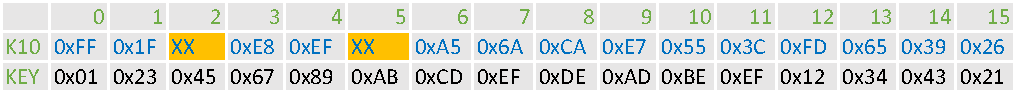
\includegraphics[width=\textwidth]{giraud__6N}
    \caption{Giraud's attack: $K^{10}$ bytes retrieved and original key}
    \label{giraudK10}
\end{table*}

After analyzing how the proposed BBI platform enhancements increase the time resolution and therefore the spatial resolution of BBI, let us now study their impact on the success of a Giraud's DFA \cite{giraud} carried out on the AES hardware coprocessor of the 32-bits microcontroller target. This DFA was chosen rather than that of Piret \& Quisquater \cite{piretQuis} since its associated fault model is more restrictive: single-bit faults are required, rather than multi-bit faults.
Furthermore, only the second and third scenarios were considered, since the impedance matching seems to be the key factor.

\begin{figure}
\centering
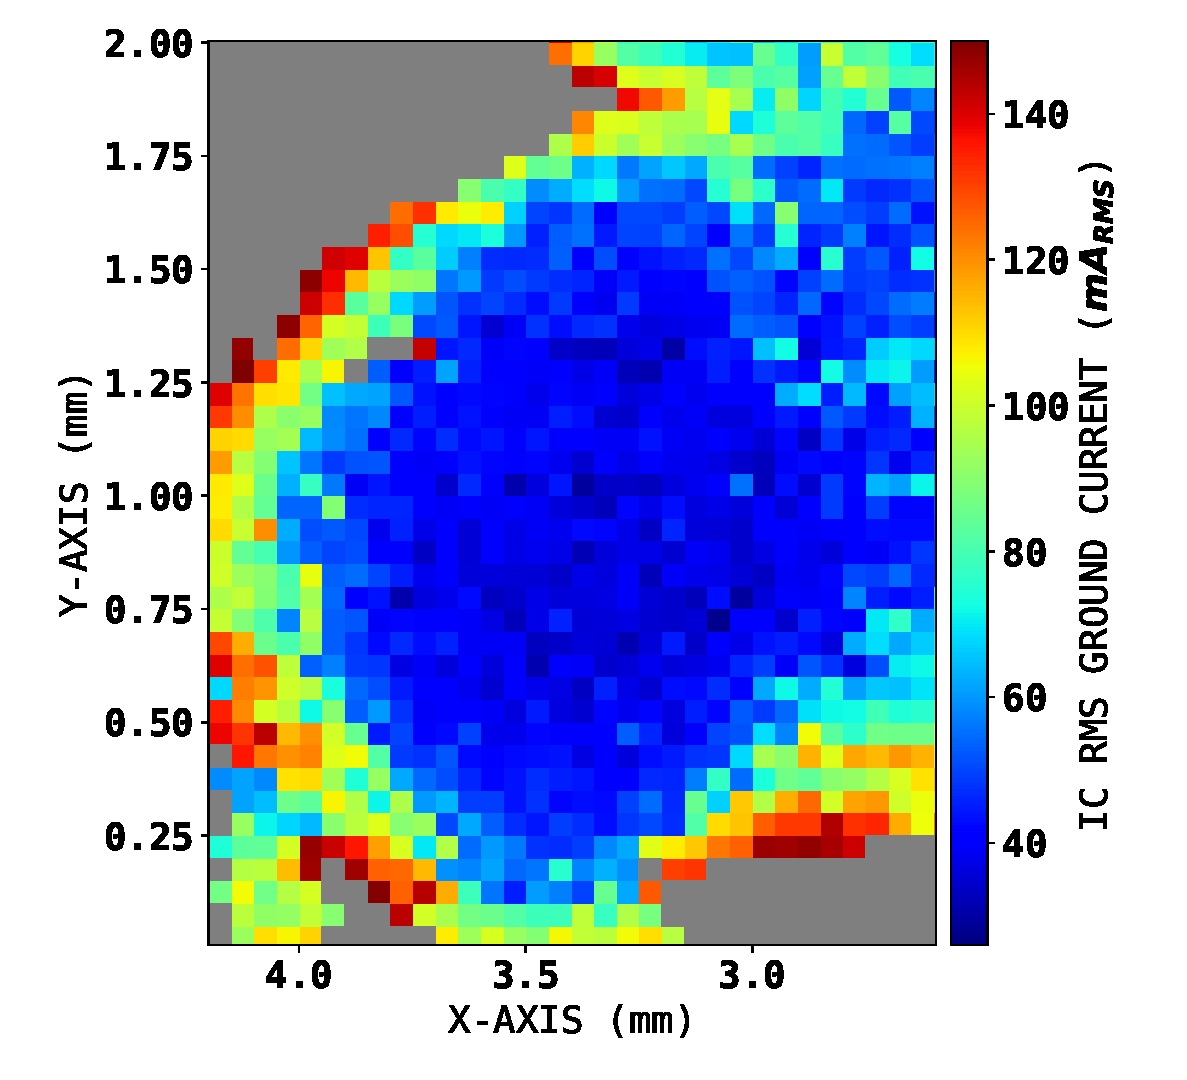
\includegraphics[width=3.3in]{GiraudAttackGoodGnd}
\caption{IC AES core fault map – Scenario 2}
\label{aesGoodGndFault}
\end{figure}

\begin{figure}
    \centering
    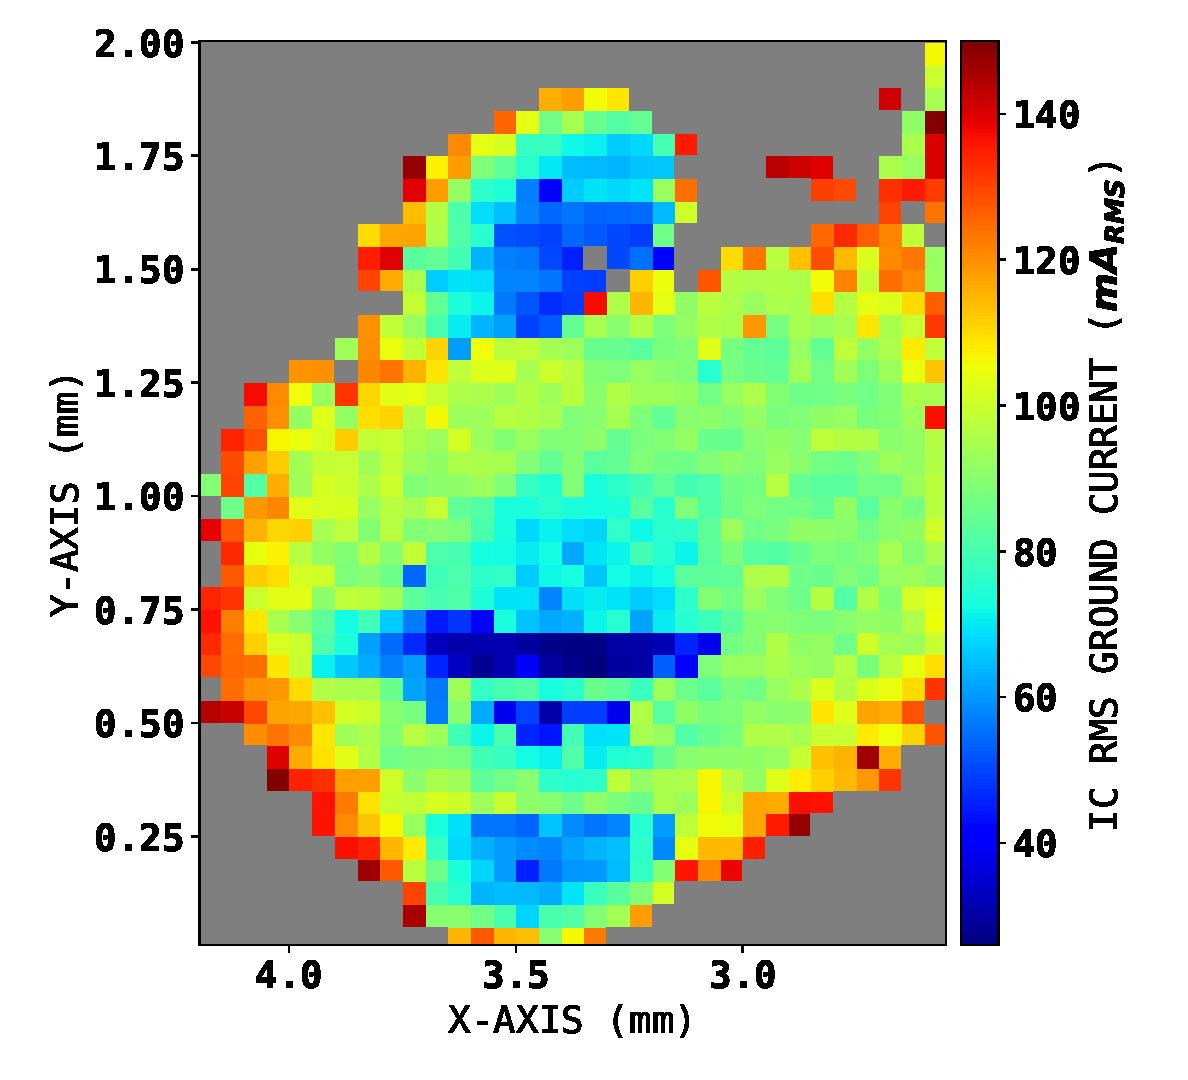
\includegraphics[width=3.3in]{GiraudAttackImpMatch}
    \caption{IC AES core fault map – Scenario 3}
    \label{aesImpGndFault}
\end{figure}

\subsubsection{IC AES core fault maps}
\label{subsubsection:aesFault}

Instead of looking for probe positions where faults meet the Giraud's fault model and performing the DFA, it was decided to perform more precise fault susceptibility maps of the area enclosing the AES. This was done to get a more complete picture of the effect of impedance matching on the success of this attack.
The results are shown in Fig. \ref{aesGoodGndFault} and \ref{aesImpGndFault}. They look extremely similar to the ones presented in Fig. \ref{rCartos_M1_fault} and \ref{rCartos_M2_fault}, as the experimental conditions were the same.

\subsubsection{Fault analysis}
\label{subsubsection:faultAnalysis}

Unlike the previous experiments, we stored with every detail the responses from the AES to analyze them.
The analysis consisted in finding all the induced faults satisfying the Giraud's fault model, this is to say single-bit faults induced on one or several bytes just before the last sub-bytes and after the last mix-columns \cite{giraud}.

It appears that all the faults obtained during the mapping performed without impedance matching (Fig. \ref{aesGoodGndFault}) are multibyte and multi-bit faults.
Therefore, the single-bit DFA proposed by C. Giraud is unusable.
On the other hand, in Fig. \ref{aesImpGndFault}, there are multiple positions where exploitable faults are observed, specifically where the required fault current was overall lower ($X\approx 3.5\;mm$ and $Y\approx 0.6\;mm$).

\subsubsection{DFA results}
\label{subsubsection:DFAres}

The previous backside area was further studied. Fine sweeps of the probe position (with a displacement step equal to $25 \; \mu m$), of the pulse amplitude (with $2 \; V$ steps) and of the injection time (with $100 \; ps$ steps) were performed.
This allowed to recover 14 bytes of the last round key without further analysis.
Table \ref{giraudK10} gives the recovered bytes of $K^{10}$ alongside the original AES key.

This result, which has been obtained without thinning the substrate, demonstrates the soundness of the proposed BBI platforms enhancements.
Indeed, to the best of our knowledge, this is the first time a DFA based on a single bit fault model was successfully performed with BBI on a hardware coprocessor.
At that point, one question emerges: what is the underlying phenomenon explaining the occurrence of such faults?

%%%%% PARTIE 4 : Modèles détaillés et plus amples explications %%%%%
\section{From more comprehensive simulation models to fault models and fault attacks}
\label{section:attacks}

\begin{figure}[!h]
\centering
\includegraphics[width=3in]{tripleWell_no_4b.png.pdf}
\caption{Electrical schematic of a standard-cell segment (SCS) in triple-well technology}
\label{stdCell}
\end{figure}

The objective of this last section is to understand the underlying phenomenons involved inside the IC under BBI.
To that end, we will study more elaborated models similar to the ones presented in \cite{mybbi1} and \cite{mybbi2}.
They allow understanding, when used simultaneously with precise logic gates models (SPICE bsim4 models), the underneath of fault creation in ICs under BBI.
% To that end, more elaborated models similar to the ones presented in \cite{mybbi1} and \cite{mybbi2} are first studied as they allow understanding, when used simultaneously with precise logic gates models (SPICE bsim4 models), the underneath of fault creation in ICs under BBI.

%%%%% PARTIE 4 SOUS-PARTIE A : Modèles standard-cells %%%%%
\subsection{Standard-cells segment models}
\label{subsection:scsModel}

As it has been first proposed in \cite{mybbi1} and improved in \cite{mybbi2}, to simulate the effects of BBI pulses inside ICs, the considered IC is split across its volume in Standard-Cell Segments (SCS), as it has been originally proposed in \cite{mathieuEMFI} concerning EMFI physical modelling.
In our case, an SCS represents an elementary tile of the overall volume of the IC of width $w$ ($30 \; \mu m$), depth $d$ ($5 \; \mu m$), and height $t_{SUB}$, the SCS height representing the IC substrate thickness.
As previously mentioned, only triple-well substrates are considered for simplicity.
Fig. \ref{stdCell} shows the electrical schematic representing the triple well SCS used in the following simulations.
We will now describe in detail each model's sections.

The section \ovalbox{1} models the silicon substrate, which is an isotropic resistive environment where the charges can flow uniformly.
As a result, it is represented by a three-dimensional network of electrical resistances, which values are calculated according to the technology used to design the considered IC.

The section \ovalbox{2} is the model of the PN junction present between the substrate and the deep N-well, in which are lithographed the P-channel MOSFETs.
It features a diode with its junction capacitance and an electrical resistance due to the thickness of the N-well (RNW).
In addition to that, the junction between \ovalbox{1} and \ovalbox{2} represents the epitaxy layer.

Section \ovalbox{3} is the NP junction between the deep N-well and the P-well (where the N-channel MOSFETs are lithographed), which shows again a diode and its capacitance, connected backwards relative to section \ovalbox{2}.
Once again, an electrical resistance models the P-well thickness (RPW).

Sections \ovalbox{4} and \ovalbox{4'} represent an average non-behavioral model of about a hundred of logic gates, where half of their transistors are off and half are on.

Then, sections \ovalbox{5} and \ovalbox{5'} are the two local metal wires ($V_{DD}$ and $GND$) powering the logic gates.

Finally, the section \ovalbox{6} represents the decoupling cells present between both $GND$ (orange) and $V_{DD}$ (red) power rails.

Eventually, one can note that the value of each component was calculated to approach the behavior of the technology node of the experimental IC.
As a result, to simulate another triple well IC built on a different technology, it is needed to re-calculate the corresponding values for the targeted technology.
However, if this IC is lithographed on another type of substrate, one must modify the proposed model as discussed in \cite{mybbi2} to match their specific needs.

%%%%% PARTIE 4 SOUS-PARTIE B : Mise en place simus %%%%%
\subsection{Setting up the simulations}
\label{subsection:simScsSetup}

On the basis that the previously presented model only represents an elementary section of an IC volume, it is needed, to analyze and predict an entire IC behavior under BBI, to create the resulting IC by interconnecting as much SCS tiles as needed.
We automated this process using custom Python scripts, creating and connecting procedurally every SPICE netlist and sub netlist.
Then, the main generated netlist was input into \mbox{Synopsys\textregistered's PrimeSim HSPICE}, and we analyzed the resulting output.

Because simulating such an IC is computationally heavy and requires a lot of memory, we decided according to the hardware available in our lab, to limit the final simulated IC size to a width of $270 \; \mu m$, a depth of $330 \; \mu m$ and a height of $100 \; \mu m$ (representing $132 \times 18 = 2376$ SCS tiles), which is way less than the experimental IC but does not cause any issue as one can evaluate the scaling of BBI effects thanks to \cite{mybbi1}.

In every performed simulation, the BBI probe used to inject the voltage pulses is located at the center of the IC and consists of a $30 \; \mu m$ square.
The applied voltage pulses are of negative polarity of amplitude $280 \; V$, of pulse width $20 \; ns$, with rise and fall times of $8 \; ns$.

Because we considered three scenarios, three simulations were performed and their result analyzed.
In each case, we specifically studied the behavior of the standard-cell segment located under the BBI probe, which is the one ideally targeted by the BBI probe.
More precisely, ten signals considered as the most important are plotted in Fig. \ref{sM0L}, \ref{sM1L} and \ref{sM2L}.
The first three signals concern the entire IC, while the seven others are specific to the targeted SCS.
These signals are, in order of occurrence, from top to bottom and from left to right:
\begin{itemize}
    \item The measured voltage pulse on the IC backside (in green),
    \item The current delivered by the voltage pulse generator (in black),
    \item The current going out of the IC ground pin (in magenta).
    \item The local SCS ground (in black), $GNDC$.
    \item The local SCS VDD (in black), $VDDC$.
    \item The current through the substrate going to the upper SCS layers (Sub $\rightarrow$ Epitaxy current).
    \item The local differential SCS power supply ($VDDC - GNDC$).
    \item The voltage at the epitaxy level.
    \item The voltage at the P-well junction.
    \item The voltage at the N-well junction.
\end{itemize}

%%%%% PARTIE 4 SOUS-PARTIE B SOUS-SOUS-PARTIE 1 : Simus SCS %%%%%
\subsubsection{\textbf{Standard-Cells electrical behavior}}
\label{subsubsection:scsExpl}

\begin{figure}[!hbtp]
\centering
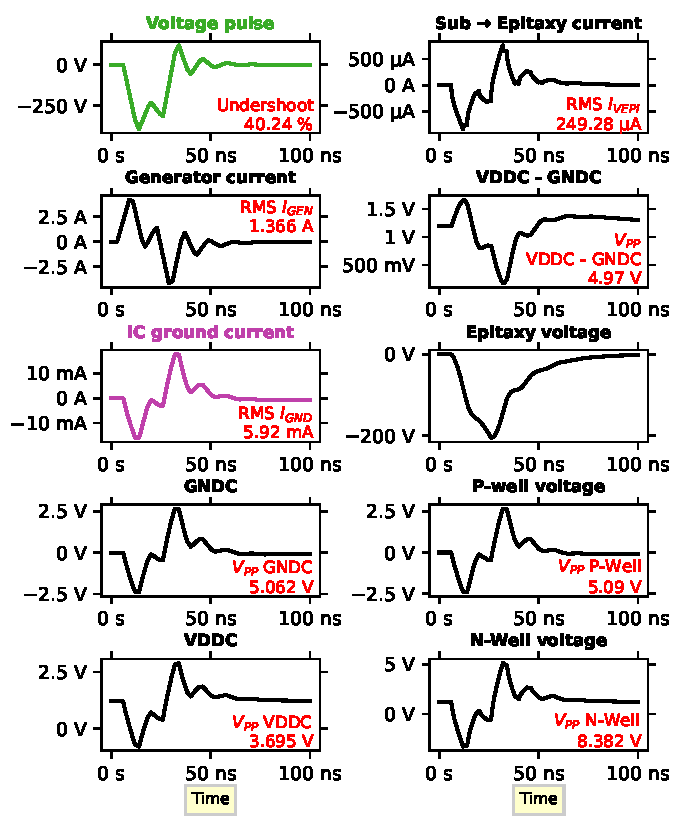
\includegraphics[width=3.3in]{latexM0_T}
\caption{Simulation results – Scenario 1}
\label{sM0L}
\end{figure}

\begin{figure}[!hbtp]
\centering
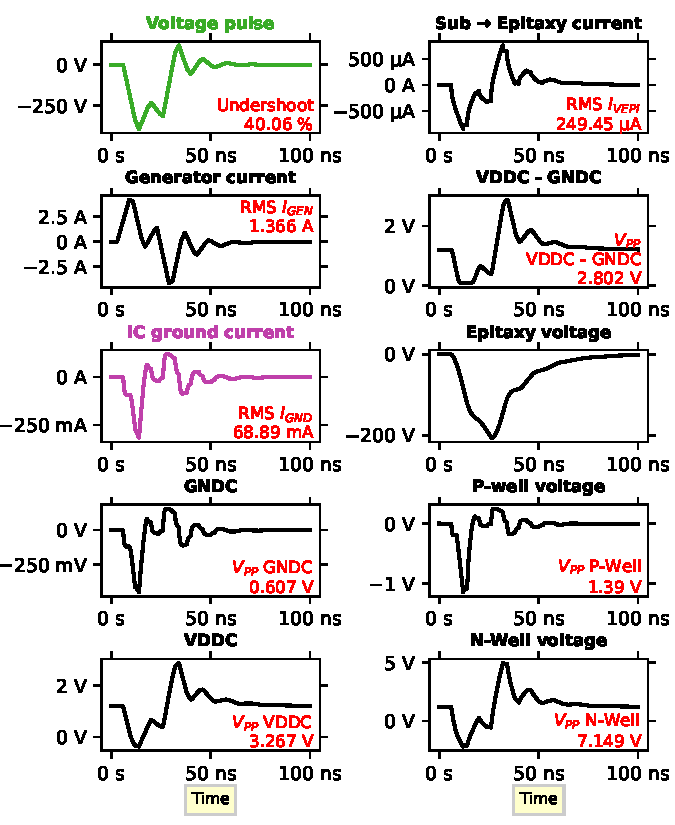
\includegraphics[width=3.3in]{latexM1_T}
\caption{Simulation results – Scenario 2}
\label{sM1L}
\end{figure}

\begin{figure}[!hbtp]
\centering
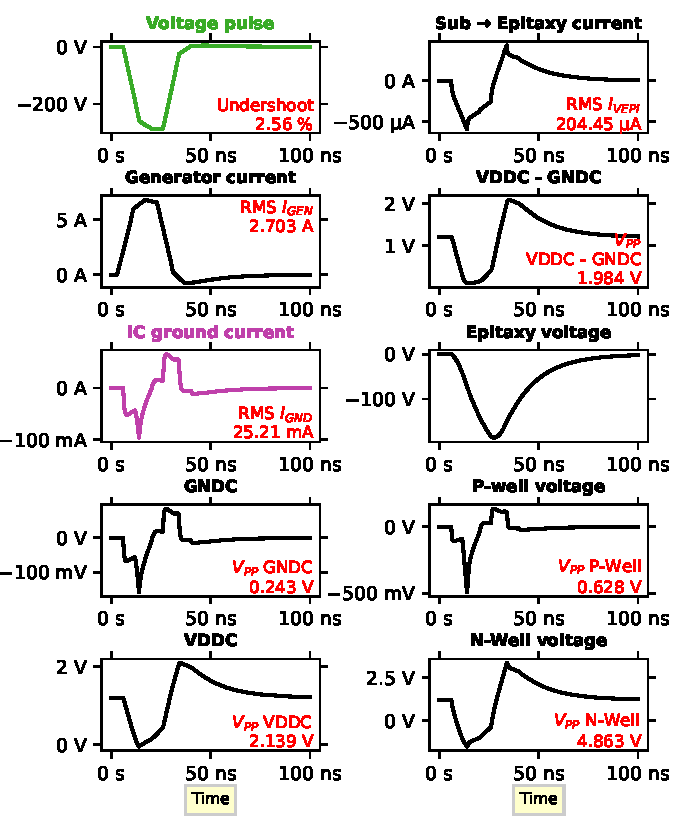
\includegraphics[width=3.3in]{latexM2_T}
\caption{Simulation results – Scenario 3}
\label{sM2L}
\end{figure}

First, as it can be observed in Fig. \ref{sM0L} and \ref{sM1L} concerning scenarios 1 and 2, the requested voltage undershoots the set-point, as it was experimented before, by about $40 \; \%$ in both cases.
In addition to this, the current of the generator exhibits large ringing as it was also expected, which is then logically echoed on the IC ground current waveforms.
However, in the first scenario (Fig. \ref{sM0L}), the amount of current on the IC ground stays fairly low (compared to the voltage sent to the IC backside), while it is multiplied by more than ten in the second scenario (Fig. \ref{sM1L}) thanks to the ground bypass.

In addition to this, the ground bypass helps a little in reducing the ringing in every internal IC signals while it stays identical in the transmission line, as it can be observed on the waveform of the current delivered by the pulse generator.

Eventually, concerning the third scenario, one can observe a significant ringing reduction, both in its amplitude and duration.
It is noteworthy concerning the applied voltage pulse and the current delivered by the generator, which are then echoed on all internal SCS signals.
This results in more precise and sharper signals, which enables for an attacker to improve both the time and spatial resolutions of its fault injections.

However, if solely observing these signals helps in understanding the previous impedance maps, it is not enough to 
properly understand the differences between the fault susceptibility maps and the underlying phenomenons of fault occurrence in ICs under BBI.
This is why in the next subsection we present the results obtained when considering CMOS logic gates under BBI.
Indeed, thanks to the results of SCS simulations, specifically the local power supply, N-well and P-well voltage waveforms, it is possible to evaluate the behavior of logic gates under BBI.

%%%%% PARTIE 4 SOUS-PARTIE B SOUS-SOUS-PARTIE 2 : Simus portes logiques %%%%%
\subsubsection{Logic gates under BBI}
\label{subsubsection:Faults ivx expl}

\begin{figure}[!hbtp]
\centering
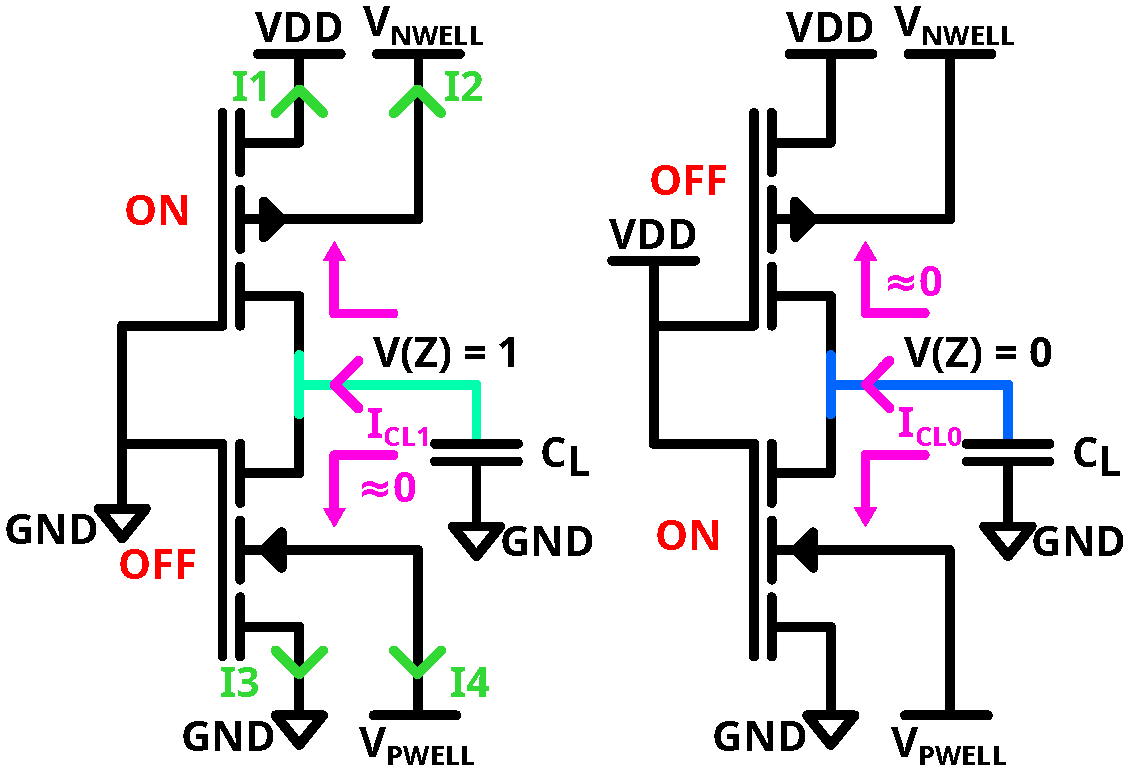
\includegraphics[width=3.1in]{ivx3New}
\caption{Simulated inverters}
\label{ivxSim}
\end{figure}

\begin{figure}[!hbtp]
\centering
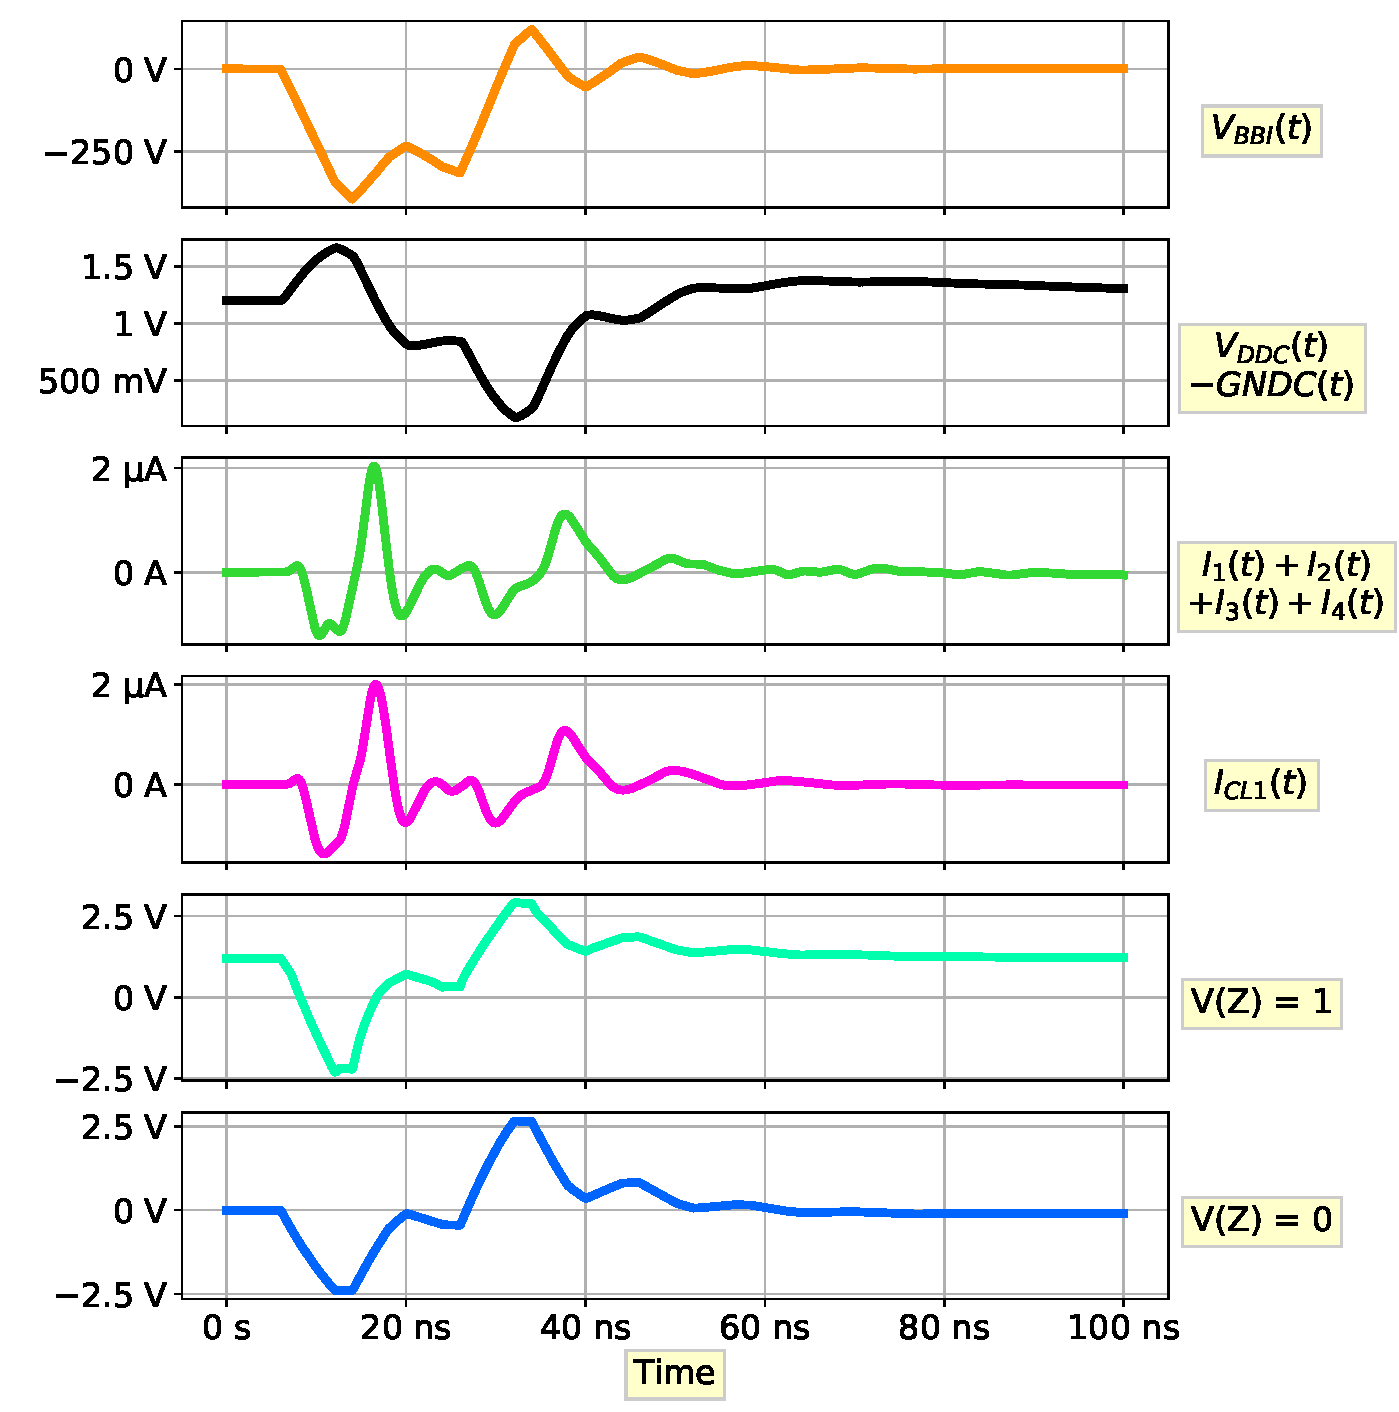
\includegraphics[width=3.2in]{logic_gates_tri_M0}
\caption{Inverters under BBI – Scenario 1}
\label{simIvxM0}
\end{figure}

\begin{figure}[!hbtp]
\centering
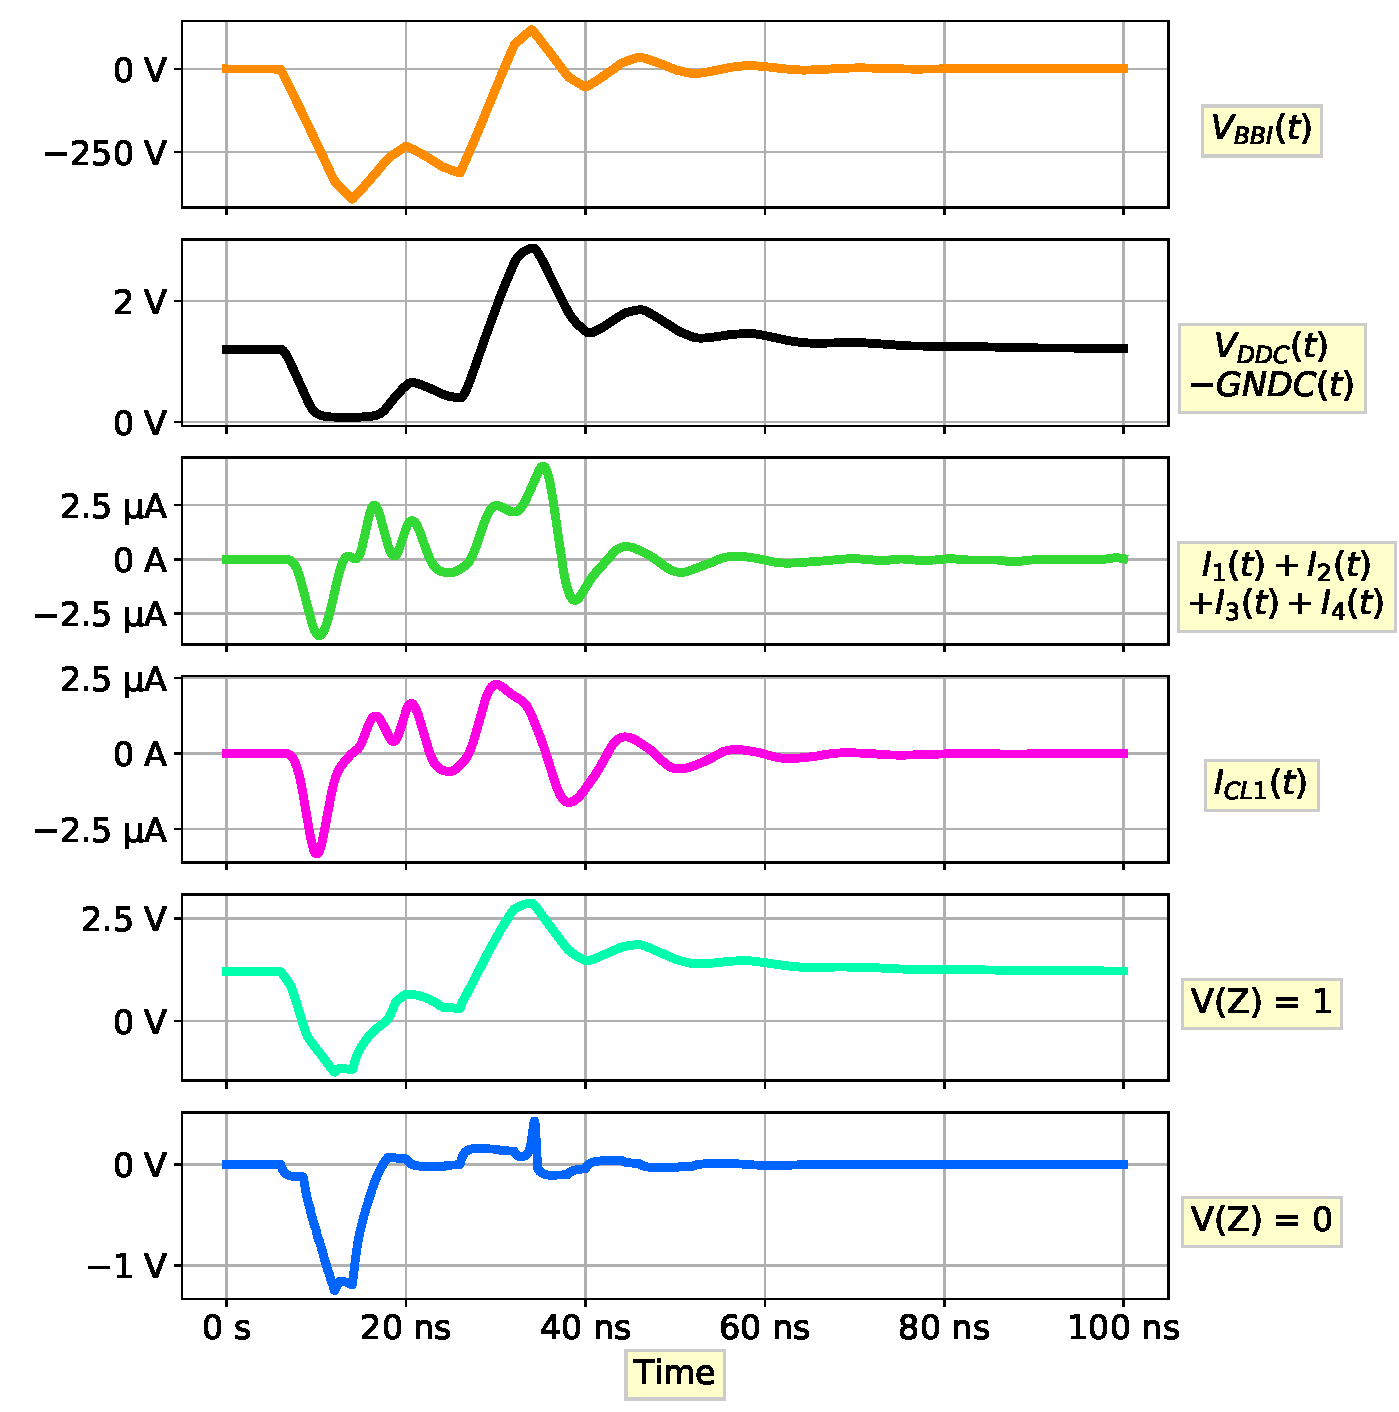
\includegraphics[width=3.2in]{logic_gates_tri_M1}
\caption{Inverters under BBI – Scenario 2}
\label{simIvxM1}
\end{figure}

\begin{figure}[!hbtp]
\centering
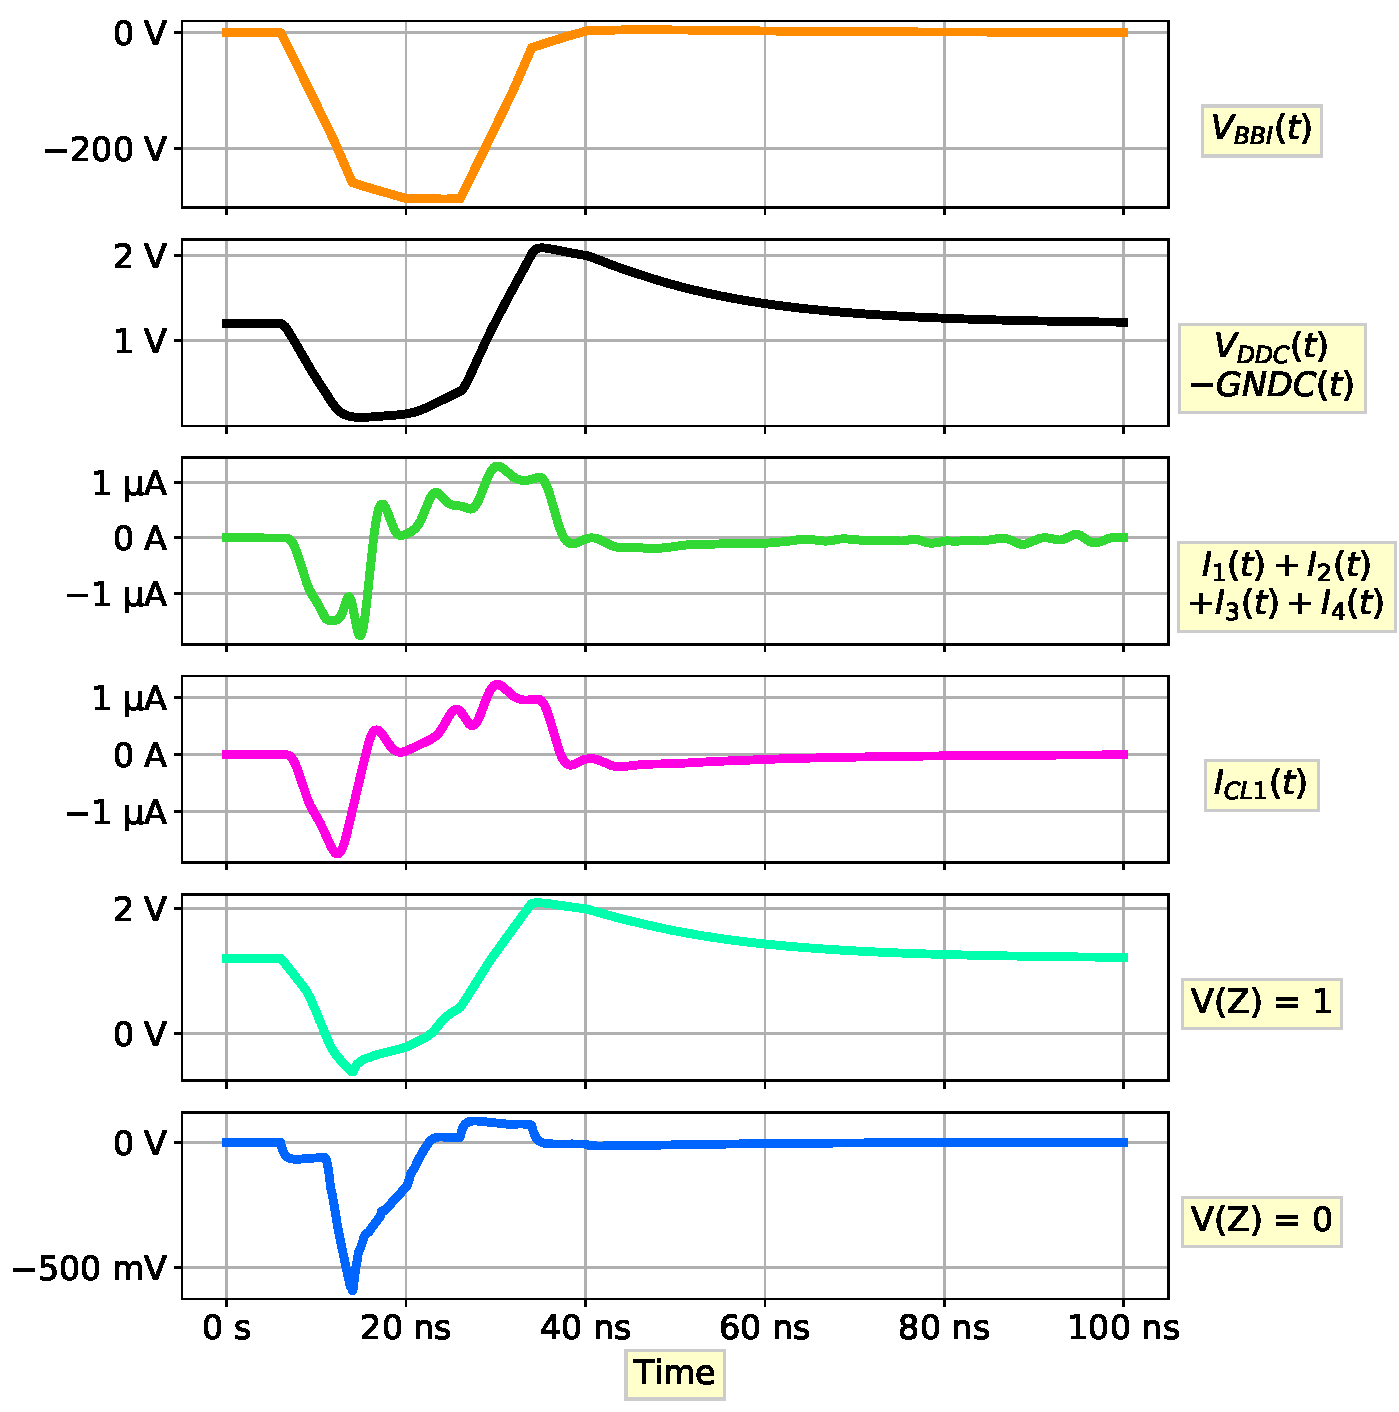
\includegraphics[width=3.2in]{logic_gates_tri_M2}
\caption{Inverters under BBI – Scenario 3}
\label{simIvxM2}
\end{figure}

To understand why faults can occur in ICs subject to BBI impulses, we decided to inject the previously simulated disturbances into CMOS logic gates.
More specifically, two inverters were simulated with the same technology node as the device under test.
Each one had a different output configuration, as shown in Fig. \ref{ivxSim}.
To that end, the disturbed signals were extracted from the SCS simulations and then reused to set the operating conditions of the inverters.
The injected signals were specifically the local power supply and the local N-well and P-well voltages.
As before, three scenarios were considered and simulated, as shown in Fig. \ref{simIvxM0}, \ref{simIvxM1} and \ref{simIvxM2}.
For each case, eight waveforms were considered in the following order:
\begin{itemize}
    \item The measured voltage pulse on the IC backside (in orange).
    \item The output voltage of a normally high inverter (in cyan).
    \item The output voltage of a normally low inverter (in blue).
    \item The differential power supply voltage.
    \item The current flowing through the normally high inverter.
    \item The current flowing through the normally high inverter load ($C_L$).
\end{itemize}
In each scenario, we can observe that the output of the inverters are pulled down during the pulse, as the generator is first absorbing carriers on the first edge (due to the negative polarity), before re-injecting them on the second edge.
This can be observed thanks to the two bottom waveforms, who are respectively the electric current through the normally high inverter and the electric current through its capacitive load.
As one can observe, the number of charges going from the substrate through the transistors, toward the ground and supply pads (which is the injected current during BBI) which is the sum of $I1$, $I2$, $I3$ and $I4$, is equal to the current of the load $I_{CL1}$.
Therefore, as shown in Fig. \ref{ivxSim}, we can conclude that the carriers stored into the logic gates loads are absorbed by the BBI probe.
On one hand, if the inverter outputs a high logical output, most of the charges flow through the VDD power network because the NMOS transistor is turned off.
On the other hand, if the inverter outputs a low logical level, most of the charges flow rather through the GND power network since the PMOS transistor is turned off.
Indeed, the charges can flow only through the conducting transistor in each case (annotated with angled magenta arrows in Fig. \ref{ivxSim}).

However, even though the inverter outputs are pulled down in all cases, the amplitude, and the duration of the voltage drop differ from one scenario to another.
In the first and second scenarios, the normally high inverter ($V_Z = 1$) experiences a drop of more than $1 \; V$.
The output voltage becomes negative and stays negative (the logical value has therefore changed) for $8.5 \; ns$ and $9.4 \; ns$ in the first and second scenarios.
Then, it quickly rises back first towards its correct value because of the ringing, to finally settle down after the second edge.
Thus, there is a transient flip of the inverter logical output value.
In the third scenario, the drop has a lower value but lasts for $11.8 \; ns$ since there is no ringing, and gets back to its correct value after $21.5 \; ns$.
The third scenario shows a clear advantage over the first two.
Indeed, the elapsed time between the fall of the output and its return to its correct value ($1.2 \; V$) is roughly equal to the width ($22 \; ns$) of the applied voltage pulse.
Hence, matching impedance allows a finer control of the voltage drop duration.
It is not the case for scenarios 1 and 2 where the ringing also influences in an uncontrolled way the voltage drop duration.

Eventually, it should also be noted that the second edge of the pulse acts similarly but inversely.
Concerning the normally low inverter ($V_Z = 0$), its output rises to more than $2.5 \; V$.
There is thus a logic value inversion lasting more or less depending on the ringing amplitude.

Overall, it seems that BBI induces faults by siphoning the electrical charges at the output of the logic gates below the probe during the first edge of the pulse to re-inject them at the second edge of the pulse.
Between the two edges, their outputs have a temporary wrong value.
If sampled at the next clock edge, they can propagate a faulty behavior in the IC architecture.

\section{Conclusion}
\label{conclusion}
Body biasing injection involves injecting voltage pulses onto the substrate of an integrated circuit.
Previous studies have examined the impact of thinning the substrate of integrated circuits, while others have demonstrated the variations in the implementation of BBI based on the substrate type.
We introduced better BBI platforms to achieve highly repeatable experiments and brought detailed insights into fault appearance inside ICs subjected to BBI.
To obtain precise faults, we observed that one should consider matching the impedance of the voltage generator.
Although it is not a novelty, it has never been studied concerning BBI.
It allows you to finely control the platform parameters, including pulse duration and set point.
Eventually, a Giraud DFA, based on a single bit fault model that is constraining, was presented on a hardware AES core, thereby demonstrating the advantages of the proposed BBI platform enhancements.


\begin{thebibliography}{1}

\bibitem{giraud}
Giraud, C. (2005). DFA on AES. In: Dobbertin, H., Rijmen, V., Sowa, A. (eds) Advanced Encryption Standard – AES. AES 2004. Lecture Notes in Computer Science, vol 3373. Springer, Berlin, Heidelberg. https://doi.org/10.1007/11506447\_4

\bibitem{optical}
Skorobogatov, S.P., Anderson, R.J. (2003). Optical Fault Induction Attacks. In: Kaliski, B.S., Koç, ç.K., Paar, C. (eds) Cryptographic Hardware and Embedded Systems - CHES 2002. CHES 2002. Lecture Notes in Computer Science, vol 2523. Springer, Berlin, Heidelberg. https://doi.org/10.1007/3-540-36400-5\_2

\bibitem{pmaurine2012}
Philippe Maurine, Karim Tobich, Thomas Ordas, Pierre yvan Liardet. Yet Another Fault Injection Technique : by Forward Body Biasing Injection. YACC'2012: Yet Another Conference on Cryptography, Sep 2012, Porquerolles Island, France. (lirmm-00762035)

\bibitem{ktobich2013}
K. Tobich, P. Maurine, P. -. Liardet, M. Lisart and T. Ordas, "Voltage Spikes on the Substrate to Obtain Timing Faults," 2013 Euromicro Conference on Digital System Design, 2013, pp. 483-486, doi: 10.1109/DSD.2013.146.

\bibitem{nbb2016}
Noemie Beringuier-Boher, Marc Lacruche, David El-Baze, Jean-Max Dutertre, Jean-Baptiste Rigaud, et al.. Body Biasing Injection Attacks in Practice . CS2: Cryptography and Security in Computing Systems, Jan 2016, Prague, Czech Republic. pp.49-54, (10.1145/2858930.2858940). (lirmm-0143414)

\bibitem{oflynn2020}
Colin O'Flynn.
\newblock Low-cost body biasing injection {(BBI)} attacks on {WLCSP} devices.
\newblock In Pierre{-}Yvan Liardet and Nele Mentens, editors, {\em{CARDIS}
2020, Virtual Event, November 18-19, 2020, Revised Selected Papers}, volume
12609 of {\em Lecture Notes in Computer Science}, pages 166--180. Springer,
2020.

\bibitem{mathieuEMFI}
M. Dumont, M. Lisart and P. Maurine, "Modeling and Simulating Electromagnetic Fault Injection," in IEEE Transactions on Computer-Aided Design of Integrated Circuits and Systems, vol. 40, no. 4, pp. 680-693, April 2021, doi: 10.1109/TCAD.2020.3003287.

\bibitem{lfitriplewell}
Nicolas Borrel, Clément Champeix, Edith Kussener, Wenceslas Rahajandraibe, Mathieu Lisart, et al.. Influence of triple-well technology on laser fault injection and laser sensor efficiency. IEEE International Symposium on Defect and Fault Tolerance in VLSI and Nanotechnology Systems (DFTS 2015), Oct 2015, Amherst, MA, United States. (10.1109/DFT.2015.7315141). (emse-01227366)

\bibitem{techEM}
P. Maurine, "Techniques for EM Fault Injection: Equipments and Experimental Results," 2012 Workshop on Fault Diagnosis and Tolerance in Cryptography, 2012, pp. 3-4, doi: 10.1109/FDTC.2012.21.

\bibitem{phototriple}
Nicolas Borrel, Clément Champeix, Mathieu Lisart, Alexandre Sarafianos, Edith Kussener, et al.. Characterization and simulation of a body biased structure in triple-well technology under pulsed photoelectric laser stimulation. International Symposium for Testing and Failure Analysis (ISTFA), Nov 2014, Houston, United States. (emse-01099035)

\bibitem{mybbi1}
Chancel, G., Galliere, J.-M., Maurine, P. (2022). Body Biasing Injection: To Thin or Not to Thin the Substrate?. In: Balasch, J., O’Flynn, C. (eds) Constructive Side-Channel Analysis and Secure Design. COSADE 2022. Lecture Notes in Computer Science, vol 13211. Springer, Cham. https://doi.org/10.1007/978-3-030-99766-3\_6.

\bibitem{mybbi2}
G. Chancel, J.-M. Galliere and P. Maurine, "Body Biasing Injection: Impact of substrate types on the induced disturbances," 2022 Workshop on Fault Detection and Tolerance in Cryptography (FDTC), Italy, 2022, pp. 50-60, doi: 10.1109/FDTC57191.2022.00015.

\bibitem{japBBI}
T. Wadatsumi et al., "Voltage Surges by Backside ESD Impacts on IC Chip in Flip Chip Packaging," 2022 IEEE International Reliability Physics Symposium (IRPS), 2022, pp. P14-1-P14-6, doi: 10.1109/IRPS48227.2022.9764457.

\bibitem{piretQuis}
Christophe Giraud and Adrian Thillard. Piret and Quisquater's DFA on AES Revisited. Cryptology ePrint Archive, Paper 2010/440, 2010.

\bibitem{powerGlitch}
L. Zussa, J. -M. Dutertre, J. Clédière and A. Tria, "Power supply glitch induced faults on FPGA: An in-depth analysis of the injection mechanism," 2013 IEEE 19th International On-Line Testing Symposium (IOLTS), Chania, Greece, 2013, pp. 110-115, doi: 10.1109/IOLTS.2013.6604060.

\end{thebibliography}

\end{document}
